\documentclass[a4paper, 10pt]{article}
\usepackage{textcomp}

\usepackage{graphicx}
\usepackage[caption=false,font=small]{subfig}

\usepackage{hyperref}
\usepackage{fancyvrb}
\usepackage{listings}

\usepackage{booktabs}
\usepackage{threeparttable} % For table with footnotes

% fun with danger signs
%\usepackage{stackengine}
%\usepackage{scalerel}
%\usepackage{xcolor}
%\newcommand\dangersign[1][2ex]{%
%  \renewcommand\stacktype{L}%
%  \scaleto{\stackon[1.3pt]{\color{red}$\triangle$}{\tiny\bfseries !}}{#1}%
%}

\usepackage{xspace}

%\newcommand{\gmadd}[1]{\textcolor{blue}{#1}}
%\newcommand{\gmadd}[1]{{#1}}

\newcommand{\ex}{\textit{IBM Exascale Extrapolator}\xspace}
\newcommand{\eb}{\textit{IBM ExaBounds}\xspace}
\newcommand{\pisa}{\textit{IBM Platform-Independent Software Analysis}\xspace}
\newcommand{\mathe}{\textit{Mathematica}\xspace}

\newcommand{\sfigbigbig}[0]{7.7cm}%{\columnwidth}
\newcommand{\sfigbigwhole}[0]{\columnwidth}%{17cm}
\newcommand{\sfigbig}[0]{7.4cm}
\newcommand{\sfigmedium}[0]{5.8cm}
\newcommand{\sfigsmall}[0]{4.1cm}
\newcommand{\sfigradarplot}[0]{4.2cm}
\newcommand{\sfigsmallsmall}[0]{2.4cm}



% make straight double quotes with \mathtt{"} in math mode
\DeclareMathSymbol{"}{\mathalpha}{letters}{`"}

\title{IBM Exascale Extrapolator manual}
%\author{G. Mariani\\IBM Research, the Netherlands}
\date{\today}

\begin{document}

\maketitle

\tableofcontents

\section{Introduction}
\label{sec:intro}
\ex is a tool for extrapolating application profiles and it is meant for predicting the behavior of application
at a scale where the actual analysis is not practical. \ex is implemented in \mathe. Users only interested in
applying the \ex tool to their own applications via its GUI do not need to have deep knowledge of the \mathe language.

\ex is tightly coupled to the \pisa profiler and the \eb analysis model. Nonetheless \ex can be used as a standalone tool
assuming that input profiles are loaded into \mathe with the expected format (Sections \ref{apx:pisaFormat} -- \ref{apx:matheAppFormat}).



The \ex framework is organized in passes:
\begin{enumerate}
 \item Loading the input datasets (Section \ref{sec:input}).
 \item Classification of thread profiles (Section \ref{sec:classification}).
 \item Setup of the extrapolation models (Section \ref{sec:setup}).
 \item Automated model construction (Section \ref{sec:construction}).
 \item Graphical model inspection and adjustment (Section \ref{sec:inspection}).\label{pass:inspection}
 \item Extrapolation and output generation (Section \ref{sec:output}).
\end{enumerate}

The overall approach is semi-automatic as Pass \ref{pass:inspection} is an interactive process where the user can
investigate graphically the extrapolation models and decide if to accept them or adjust them to meet user's expectations.
In practice, Pass \ref{pass:inspection} could be skipped but, as observed by Mariani et al. \cite{mariani2015cf}, large deviations
of the predicted metrics can be found when the model selection is fully automated with no user inspection. The
observed deviations when analyzing the SPEC CPU 2006 have been demonstrated of up to an order of magnitude from the actual
metric value. These deviations can even grow when extrapolating farer from the
training region.

The reminder of this documentation is organized as follows. Section \ref{sec:semiauto} clarifies the importance of a
semi-automated approach by explaining how noises in the training data can lead to unacceptable deviations of the extrapolation
model from the actual metric when a fully-automated approach is used. Then, Section \ref{sec:beginning} describes
how to setup an \ex project such to enable the user to save and load partial results. The document continues with Sections
\ref{sec:input}--\ref{sec:output} to describe each pass of the \ex methodology. Finally, Sections \ref{sec:contributors}
and \ref{sec:ack} list the contributors and acknowledge the funding sources.


\section{Why a semi-automatic approach?}
\label{sec:semiauto}

The extrapolation methodology implemented in \ex is a delicate procedure based on machine learning. Minor noises in the training
data for a target metric may lead to the construction of prediction models whose trend diverges from the trend of the actual target metric.
In fact these noises can lead to minor perturbations on the learnt model coefficients that might generate unreasonable deviation
from the target metric as we get far from the training region.

For example, let us consider that we try to learn a model for a metric $y$ that is a linear function of $x$:
\begin{equation}
 y = c_0 + c_1 x
\end{equation}
The prediction model is an approximate regression model: $\hat{y}\sim y$.
Let us assume that, by mistake we choose to use a second order model:
\begin{equation}
 \hat{y} = \hat{c}_0 + \hat{c}_1 x + \hat{c}_2 x^2
\end{equation}


In this case, minor noises in the training data might lead to an estimation of $\hat{c}_2$ that is close to zero but different from it.
The resulting model will still have a good fit in the training region because $\hat{c}_2$ is actually small enough to let
$\hat{c}_2 x^2$ be negligible when $x$ is in the range of values of the training region.
Nonetheless, this close-to-zero second order coefficient $\hat{c}_2$ will lead to a larger and larger deviation of $\hat{y}$
from the original linear trend of $y$ when $x$ grows toward the target extrapolation scale.

To overtake this problem, \ex systematically takes into account crossvalidation and statistical hypothesis testing
during model construction to avoid the introduction of misleading terms in the automatically generated models.
However:
\begin{itemize}
 \item Crossvalidation is a way to estimate model accuracy by actually predicting the target metric on
the same training set itself. This is obtained by iteratively removing some elements from the training set such as to fairly
generate predictions on these left-out elements.
Thus model construction based on crossvalidated data is a fair approach when the training set is a good representative of
the target predictions (i.e. when interpolating). When predicting far away from the training region (extrapolating),
crossvalidation can still be misleading.
 \item Statistical hypothesis testing can accept errors with a low probability (related to the confidence level used in the test).
 When constructing a model for a target metric \ex will test several different model options. Additionally, when several metrics need
 to be predicted the model construction is carried out
 for each metric. A low probability of accepting an error for a single
 hypothesis test still lead to a not-so-low probability of accepting a wrong model for some of the metrics.
\end{itemize}

Thus, regardless to the careful model selection procedure, a fully automated model construction process may lead in some cases
to low accuracy when extrapolating far from the training region due to the possibility of accepting a wrong model.
For this reason we recommend a semi-automated model selection strategy. We recommend:
\begin{itemize}
 \item Use two datasets, one for constructing the model and the other for validating it (Section \ref{sec:input}).
 \item Specify the available knowledge on the expected metric trend (Section \ref{sec:setup}).
 \item After the automatic model construction (Section \ref{sec:construction}), inspect the models graphically and discard any
 model whose trend significantly differs from the expected one (Section \ref{sec:inspection}).
\end{itemize}


\section{Before to start}
\label{sec:beginning}
Some of \ex's passes can be lengthy. In few cases when constructing models for many metrics for many
thread classes and/or when trying to process different applications during the same \mathe session,
we may experience that memory usage from the \mathe kernel increases and, in critical cases, \mathe
may run out of memory and stop working. To avoid data loss and to avoid to rerun the same computations,
we can setup an \ex project folder and then save and load data for each pass.
The project setup is done in the Section \textbf{Pass 0: Project setup} of the \ex notebook (\verb!ExtrAx.nb!).
In the same Section we can see the status of previously saved data.

When saving data for the \ex pass \verb!n!, a file named \verb!pass<n>.m! is generated to store the \mathe data
generated by the \ex pass.

\section{Loading input profiles}
\label{sec:input}

In Section \textbf{Pass 1: Reading input profiles} of the \ex notebook, we can load the application profiles for training and testing
the model. Train data is mandatory and we should load it before proceeding towards next \ex passes.
Test data is not mandatory but strongly recommended to help in the model inspection, i.e. to verify if the automatically generated models
are suitable for the application under analysis.

To load the data, first setup the folders where to find the JSON profiles for train and test. Path to these folders can be given
as absolute system path or as relative path with respect to the \ex project folder. After setting these paths, we should set the file extensions
for the train and test data. All files terminating with the selected extension in the selected folder are loaded when clicking the
\verb!Load profiles! button.

Each input profile file should be in line with the format described in Appendix \ref{apx:pisaFormat}. An
input file stores profile information for all threads executed during a single application run. Different input files store profile
data of different application runs carried out at fir different configurations of scaling parameters.

In theory, different input files may store execution of different applications.
Thus we are required to select a target application among the loaded ones.
Once the files are loaded and the target application name is selected we can backup our data with the \verb!Backup pass1! button.
We can reload the data at any time by using the \verb!Load data for pass1! button.



\section{Thread classification}
\label{sec:classification}

A parallel application is organized in threads that can implement different functionalities or process different data.
These threads can thus behave differently and extrapolation models can be necessary for matching their differences.
To cope with this issue \ex applies thread classification to identify threads that behave similarly across different
runs of the application. Then extrapolation models will be generated for each thread class.
In the Section \textbf{Pass 2: Thread classification} we can setup and execute the classification.

First we setup the classification method. Then we specify the number of classes to be found
(keep the default \verb!Automatic! option if we want the classification to automatically find the best number of classes to be used).
Once these classification options have been setup, click the \verb!Classify! button to execute the classification.
The classification process should be quite fast, it might take about ten-fifteen minutes in some cases but it usually take less then two
or three minutes. Once the classification is completed we can save the results with the backup button and optionally we can visualize them.

The classification is learnt on the training data only. If test data has been loaded, this will not influence the classification result.
Nonetheless, if test data is available, the classification learnt on the train profiles is applied to the test runs
such as to organize threads using the same classes.

\textbf{Note: the implemented classification methods assume that in each profiled run, each thread class is represented by at least one thread.
Do not include neither in the train nor in the test runs any execution with fewer threads than the potential classes we may
expect to find in the application.} For example in an MPI application where the processes are orga

\subsection{Classification methods}

There are two classification methods implemented in \ex: \texttt{General communication and processing analysis}, and
\texttt{Communication pattern regularity analysis}.

\textbf{General communication and processing analysis.} This is an unsupervised machine learning technique that carries out
an independent thread clustering for each application run. All metrics in the application profile including take part in the classification
including both communication and computation related metrics.
Before clustering, the thread profile dimensionality is reduced
by applying PCA (Kaiser's criterion is applied to decide the best number of PCA dimensions to use). The number of clusters
to use is equivalent to the number of classes and, if it has to be selected automatically, it is set such to optimize the
silhouette heuristic along the different clustering.

Once the clustering is carried out for each application run, \ex associate a class to each cluster. First classes are defined by enumerating
the clusters observed in the first application run. Then, to each following application run, classes are associated to clusters
by minimizing the distance of the average profile of the cluster to other previously classified classes in other runs.

Details on this methodology are described by Mariani et al. \cite{mariani201Xclassification}.

\textbf{Communication pattern regularity analysis.} This technique identifies regularities in the communication pattern
and classifies each thread depending on the region in the communication graph the thread belongs. It can be applied only
to MPI application with a regular communication pattern. The implemented algorithm has been tested for communication graphs organized with
the following topologies: all to all, ring, 2D mesh, 3D mesh, and torus. Other regular communication patterns could be handled
but this is not granted.

The classes found with this methodology are in practice the communication groups described by Wu et al. \cite{wu2012}.
$\\$

While the first classification method can be applied to any application,
the second one has stringent requirements and cannot handle many applications.
Nonetheless, when the second method can be applied, it is usually a better option because automatic unsupervised machine learning can 
misclassify some of the threads. While classification accuracy has been proved very good \cite{mariani201Xclassification},
the noise introduced by classification error can significantly reduce the accuracy of the extrapolation model that are trained
on some misclassified data.

\subsection{Visualization of classification results}
Once the classification is organized, the results can be visualized by clicking the button \verb!Show results!. Note
that to visualize the results might take few minutes and also the graphics may be automatically refreshed by \mathe
while working on other sections of the \ex notebook. We recommend to hide the graphics before proceeding to next passes.

At the top of the classification visualization we can select the metrics to be visualized from a control grid named
\textbf{Visualized metrics} (Figure \ref{fig:clusteringMetricSelection}).
If the classification is carried out by using the \texttt{General communication and processing analysis} method,
it is possible to visualize the classification results in the principal component space representation by selecting
the option: \verb!principal component analysis!. After modifying the metrics to be visualized, click \texttt{Refresh}.


\begin{figure}[h!]
\centering
\resizebox{\sfigbigwhole}{!}{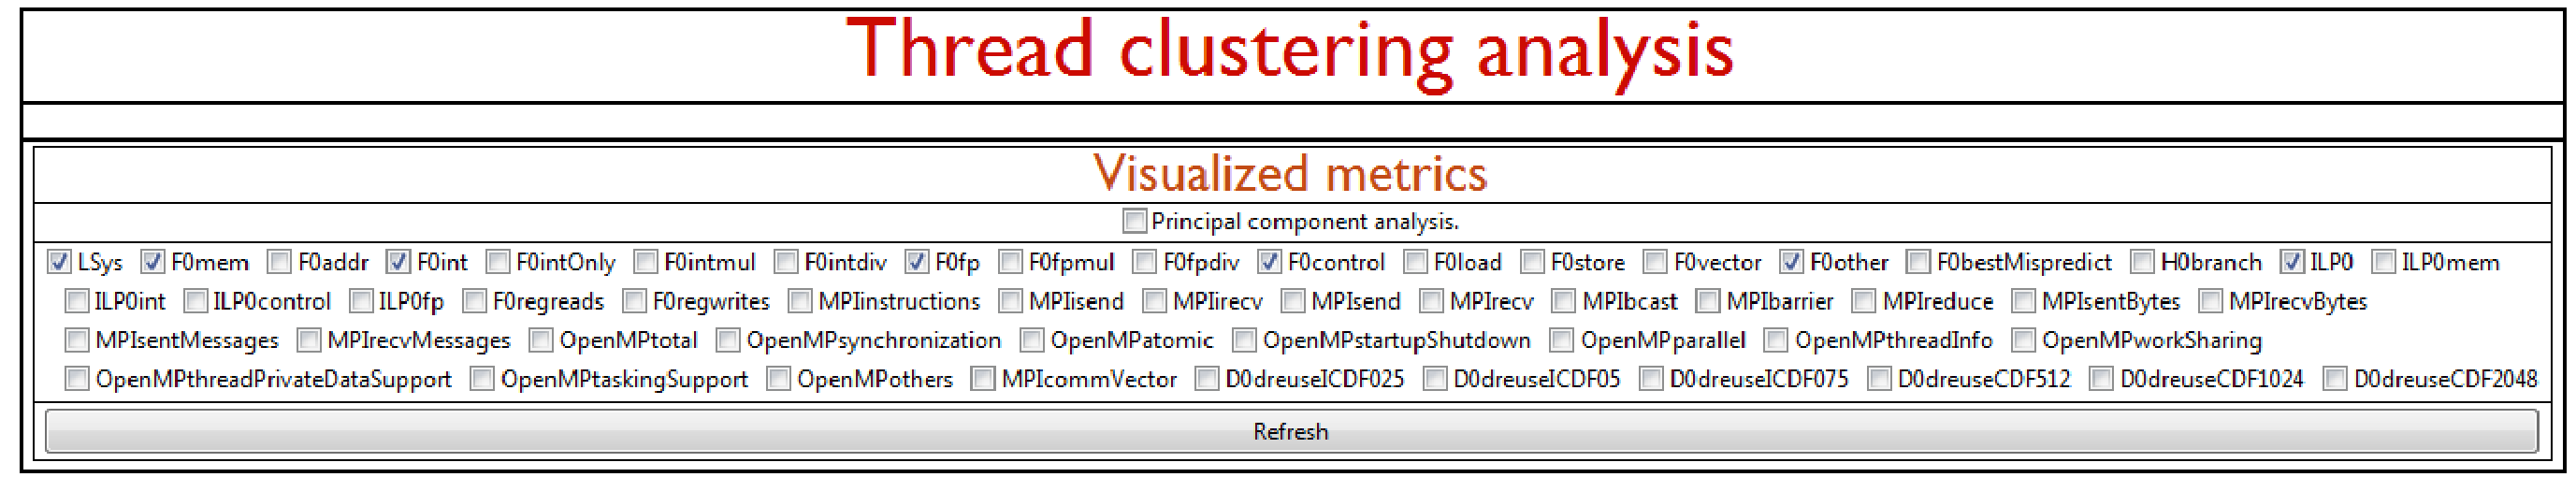
\includegraphics{./Figures/clusteringControlGUI.pdf}}
\caption{Interface to select the metrics for the class visualization.}
\label{fig:clusteringMetricSelection}
\end{figure}

The clustering is visualized in a table format using radar plots. Thick blue lines are used to highlight the
average class metrics while thin green lines show the behavior of each thread in a given class.
Rows of the table corresponds to runs of the application
and are entitled with the corresponding scaling configuration. Classes are visualized with radar plots that show the value
of the selected metric for the given class. Classes are automatically named alphabetically starting with \verb!A!
and are assigned with colors. In the case of MPI application using peer to peer communication, the communication graph
is visualized for each application run. Vertices of the communication graph are colored accordingly to the class assigned
to thread classification. Figure \ref{fig:clusteringVisualization} shows the classification of the first two runs in the
training set for an application using a 2D mesh communication layout. The specific classification is obtained with the
\texttt{Communication pattern regularity analysis} method.


\begin{figure}[h!]
\centering
\resizebox{\sfigbigwhole}{!}{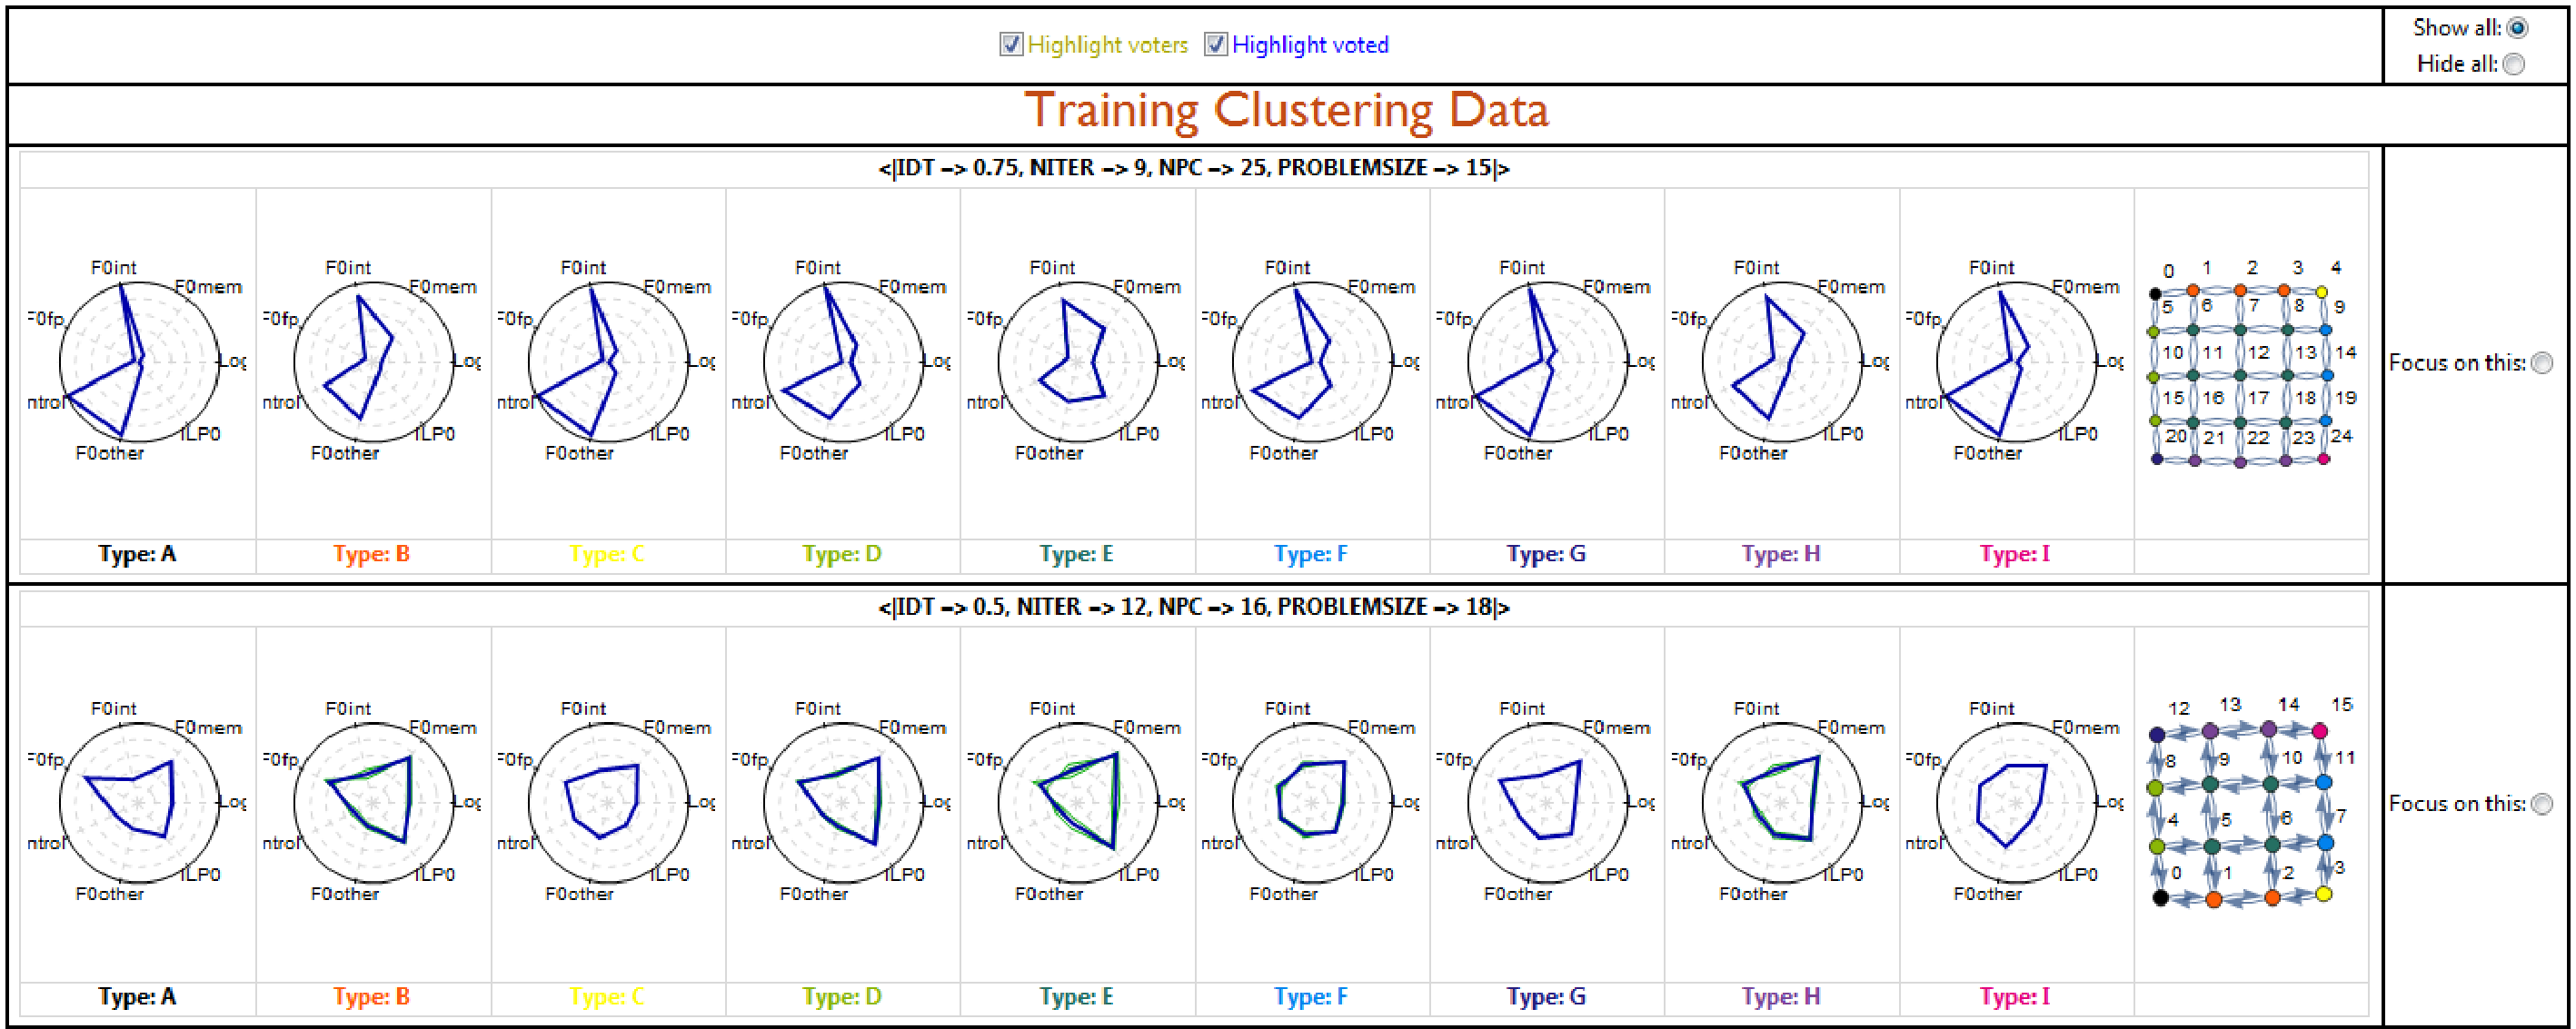
\includegraphics{./Figures/clusteringVisualization.pdf}}
\caption{Visualization of classification results.}
\label{fig:clusteringVisualization}
\end{figure}

Note that, when using the \texttt{Communication pattern regularity analysis} method, the classes
are \textit{aligned} along different runs by using a voting scheme as described in \cite{mariani201Xclassification}.
The voting scheme let propagate a unique class definition (i.e. ordering of the radar plots in a scaling configuration)
by comparing the classes found to application runs in neighboring scaling configurations.
By using the radio buttons on the right of the table, the GUI allows to focus on a given scaling configuration such to hide
all other configurations except those that were either involved in voting for or have been voted by the selected run.
This mechanism has effect only when the \texttt{Communication pattern regularity analysis} method is used.



\section{Setup the extrapolation models}
\label{sec:setup}

Before to generate the extrapolation models we need to list the metrics target of the extrapolation.
\ex then generates an extrapolation model for each of the target metric and for each thread class.
During model construction, \ex tries to find a set of terms (functions of scaling parameters)
that maximizes the model accuracy. The terms are selected by using the methodology presented by Mariani et al.
\cite{mariani2016ijpp} that requires a list of complexity definitions.

In the Section \textbf{Pass 3: Setup extrapolation methods} of the \ex notebook a GUI implements
the functionalities to manipulate the complexity definitions and the list of target metrics.

\subsection{Complexity definitions}
\label{sed:complexities}

Many of the metrics to be extrapolated can be subject of theoretical analysis for understanding the overall complexity in terms
of $\mathcal{O}$ notation of the application \cite{mariani2016ijpp}. To help the model construction we can list a set of terms that we
expect could be found when scaling the application execution. We should list these terms using the \verb!Order of complexity definitions!
input field. These are considered as the \textit{main terms} options for the model construction, as described in \cite{mariani2016ijpp}.
\textit{Interaction terms} -- i.e. combinations of different main effect terms each applied to different scaling parameters --
will automatically be considered. Additionally also the concepts of
\textit{parallel} and \textit{sequential} are handled automatically \cite{mariani2016ijpp}.

Thus in the \verb!Order of complexity definitions! we only have to list the possible main complexities. Starting from the overall
complexity $\mathcal{O}$ we may include expression that may grow slower than $\mathcal{O}$ if we expect those terms to be relevant
for the accuracy of the model. For example, if we expect the number of instructions to scale as $\mathcal{O}(n^2)$, we may want to include also
$n$ in the complexity definition because when including both $n$ and $n^2$ in the overall model we may improve the
overall accuracy with respect to a model that includes only $n^2$.

The main terms to be considered are defined using a \mathe association. In particular, we need to map the metric names (keys of this association)
to the terms to be used for that metric. To avoid repeating the same terms for each different metric
the key \verb!Automatic! can be used to set the default terms for all metrics that do not appear as key of the association.

The following example:

\verb!<|"NThreads" -> ({NPC} &), Automatic -> ({N[s]^3, N[s]^2, N[#1]} &)|>!

means that the metric \verb!"NThreads"! can scale as a linear function of \verb!NPC! and that all other metrics can scale
as the cube or square of \verb!s! and as a linear function of any scaling parameter.

\subsection{Listing the target metrics}
\label{sec:mListEdit}

We enter all the target metrics in the extrapolation list using the table available in Section \textbf{Pass 3: Setup extrapolation methods}
(Figure \ref{fig:extrapolationList}).

\begin{figure}[h!]
\centering
\resizebox{\sfigbigwhole}{!}{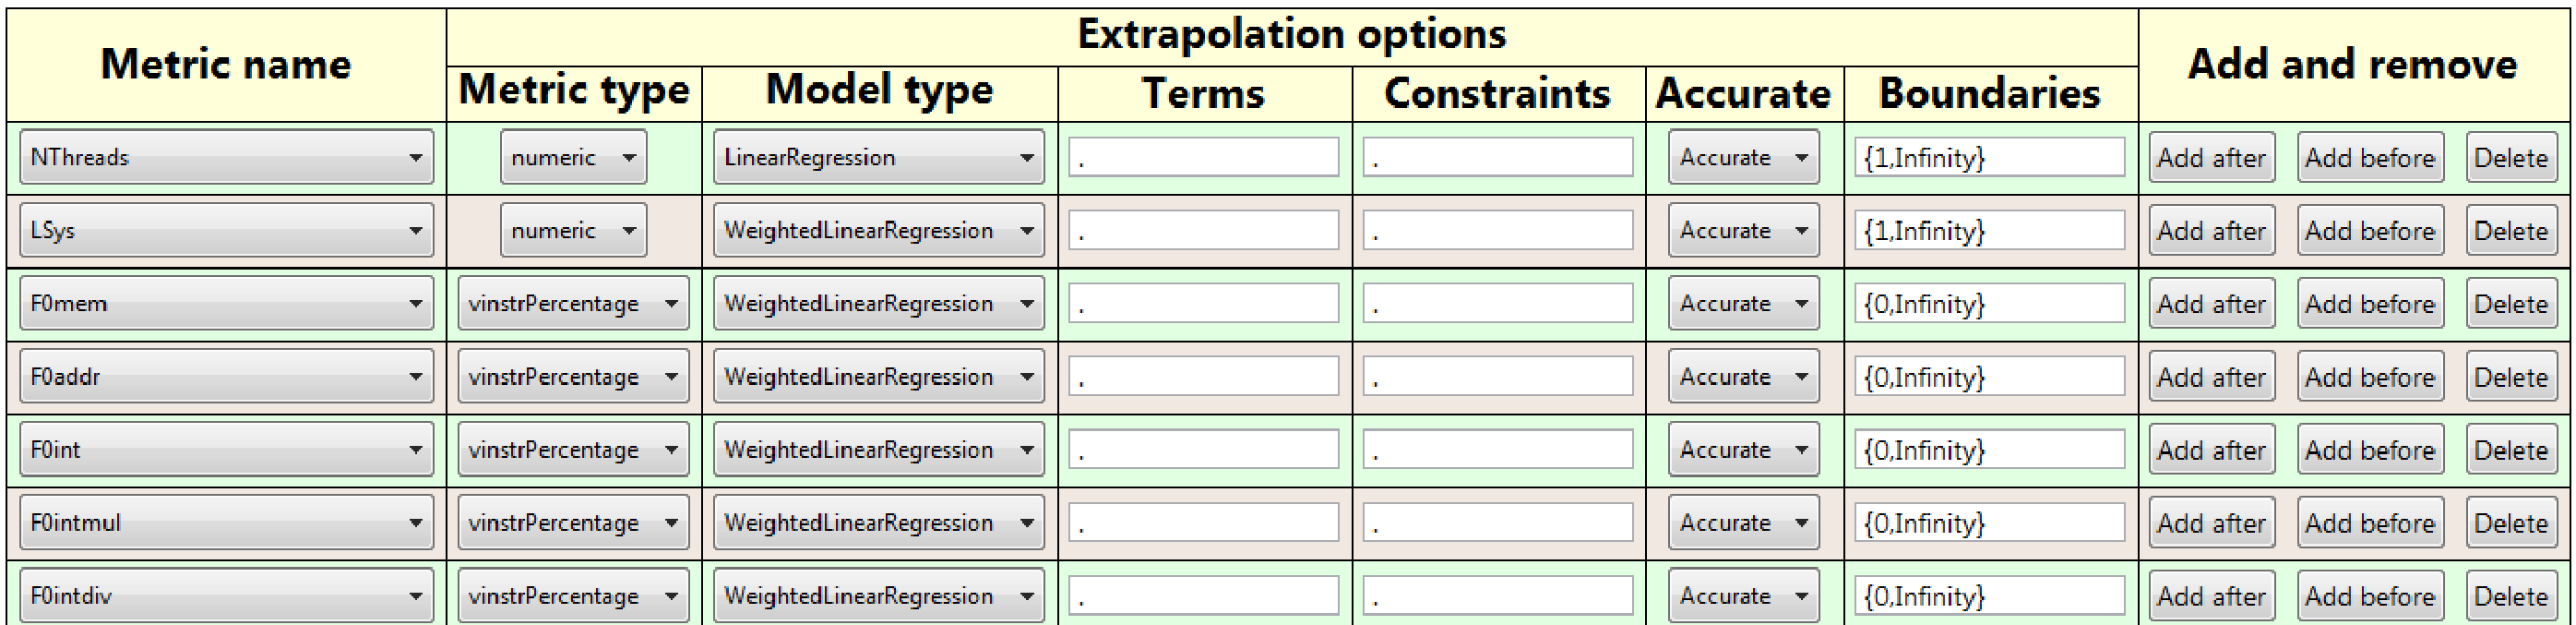
\includegraphics{./Figures/ExtrapolationListEdit.pdf}}
\caption{List of the target extrapolation metrics and parameters to be used for model construction.}
\label{fig:extrapolationList}
\end{figure}

The table is preliminary set up to list all metrics that are required by the \eb model. To add or remove metrics, use the buttons on the last column.
Metric names on the left most column have a color coding. Black means that the metric has a type known to \ex.
Orange means that the metric type is unknown to \ex but, if the user knows it, that metric could be handled by \ex
(this enables the user to handle any new metric by simply including it in the thread profile
and list it as a target metric).
Red means that some problems with that metric have been detected, e.g. the metric appears twice in the list of target metrics 
or some thread profiles do not store the metric value or it is explicitly listed in \ex as not supported
(a list of the known metrics is given in appendix \ref{apx:metricList}).

Note that the extrapolation models of some metrics require first a
model for \verb!NThreads! (the number of threads in the class),
and \verb!LSys! the total number of instructions executed. \textbf{It is recommended to always keep these two metrics at the beginning of the list.}
For each metric, a set of options for the model construction is available.

\subsubsection{Metric type}
\label{sec:mType}

The \textit{metric type} indicates the structure that a metric has and its dependence or independence from \verb!LSys!.
There are three basic types whose \mathe data structures are described in \ref{apx:matheMetricFormat}.

First, \textit{scalar} metrics are those metrics that, for each thread profile, are a scalar number.

Second, \textit{vectorized mix} metrics describe how the instructions of a given type
are distributed in terms of vectorization and data length. For each combination of vector and data lengths, a scalar number is stored
in each thread profile. All those scalar numbers have to be predicted for a \textit{vectorized mix} metric.

Third, \textit{memory functions} metrics describe a cumulative distribution function of memory reuse distance.
These metrics depends on the scaling parameters and the data reuse distance itself (this parameter is named in \ex \verb!memX!).
For \textit{memory functions} metrics the \textit{metric type} option has to be set to \textbf{memFunction}.

In \ex the \textit{scalar} and \textit{vectorized mix} metrics can be considered as either independent or dependent from \verb!LSys!.
For independent metrics, the \textit{metric type} option has to be set to \textbf{numeric} or \textbf{vnumeric}
respectively for \textit{scalar} and \textit{vectorized mix}. For a metric \verb!m! considered \verb!LSys! dependent,
we do not construct a model directly for the value stored for \verb!m! in the thread profiles but we construct
the model for the product \verb!LSys!$\times$\verb!m!. In this case
we should set the metric type option as \textbf{instrPercentage} or \textbf{vinstrPercentage}
respectively.

For example, the metric $F0int$ is the fraction of {integer} instructions profiled by \pisa. Let us assume for simplicity in this example
that $F0int$ is a scalar metric encoded with a single number for each thread profile.
First of all, we expect $F0int$ to be bounded: $0\leq F0int \leq 1$ (0 no integer instructions executed, 1 only integer instructions executed).
When predicting $F0int$ as \textbf{numeric}, we directly construct
an extrapolation model: $\widehat{F0int}\sim F0int$. When using linear regression, the model $\widehat{F0int}$ will be a linear combination
of a set of terms, for example $\widehat{F0int}=c_0 + c_1 \times x_1^3 + c_2 \times x_2$, where $x_1$ and $x_2$ are two scaling parameters,
the coefficients $c_i$ are found using linear regression, and the terms' exponents are selected using model construction.
The resulting model is unbounded and its predictions will eventually be unreasonable (outside the expected boundaries)
when changing $x_1$ and $x_2$ far away from the
training region. Nonetheless if we specify $F0int$ as \textbf{instrPercentage}, we do not construct the model for $F0int$
but for a surrogate metric $C0int=F0int \times LSys$, that is the total count of integer instructions. The model
construction will not search for the terms to be used for $\widehat{F0int}$ but will assume that the same terms used for $\widehat{LSys}$
are to be used also for $\widehat{F0int}$. For example, if $\widehat{LSys}=k_0 + k_1 \times x_1^3 + k_2 \times x_2$,
then $\widehat{C0int}=c_0 + c_1 \times x_1^3 + c_2 \times x_2$ where the parameters $c_i$ and $k_i$
are estimated via linear regression and the terms in the linear combination are selected during the model construction for $LSys$.
Then, $\widehat{F0int}=\widehat{C0int} / \widehat{LSys}$:
\begin{equation}
 \widehat{F0int} = \frac{c_0 + c_1 \times x_1^3 + c_2 \times x_2}{k_0 + k_1 \times x_1^3 + k_2 \times x_2}.
\end{equation}

$\widehat{F0int}$ is a bounded function for growing values of any of the scaling parameters
(except when $\widehat{LSys}$ returns zero for some value of interest of the scaling parameters,
see Section \ref{sec:Constraints}). This model cannot diverge infinitely from the actual trend because the difference between the asymptotes
of $\widehat{F0int}$ and the actual bounds of $F0int$ is by construction a finite number.

For all metrics that are expected to be bounded (besides the \textit{memory functions} metrics) we suggest to always use
one of the following combinations of options:
\begin{itemize}
 \item {metric type} \textbf{instrPercentage} (or \textbf{vinstrPercentage}), {model type} \textbf{WeightedLinearRegression},
 \item {metric type} \textbf{numeric} (or \textbf{vnumeric}), {model type} \textbf{NeuralNetwork}
\end{itemize}

\subsubsection{Model type}
\label{sec:modelType}
For the metric types \verb!instrPercentage! and \verb!vinstrPercentage!, only two model types are available.
These are the \textbf{WeightedLinearRegression} and the \textbf{LinearRegression}. The \textbf{WeightedLinearRegression}
applies linear regression while compensating for possible heteroscedasticity 
by applying a weighting scheme on the residual errors as suggested in \cite{mariani2016ijpp}.
The \textbf{LinearRegression} does not include any heteroscedasticity compensation and it is a straightforward linear regression.

For the metric types \verb!numeric! and \verb!vnumeric!, there are the following additional model types:
\textbf{NearestNeighbors}, \textbf{NeuralNetwork}, and \textbf{RandomForest}. These models 
simply use the machine learning functionalities of \mathe
and their default options are used. It is possible to modify their options by editing the variable \verb!defaultModelTypeProperties!
defined in the package:

\verb!AlgorithmExtrapolation/SingleThreadExtrapolation.m!

For a \verb!memFunction! (e.g. $D0dreuse$) we can generate an
approximate model ($\widehat{D0dreuse}$) as a function of the scaling parameters, the memory reuse distance \verb!memX!
and the surrogates of \verb!memX! (Section \ref{sec:terms}) by using any of the previously listed models.
% Additionally we can also generate a prediction model to predict the CDF for each different value of the memory reuse distance \verb!memX!,
% where each of these models depend only on the scaling parameters.
% This approach is similar to the one proposed by Marin et al. \cite{marin2004}.
We also have two additional model types: \textbf{PerBinLinearRegression}, and \textbf{PerBinNeuralNetwork}.
If one of these is selected, the terms cannot be dependent on \verb!memX!. The overall prediction model in this case
will be the aggregation of several prediction models, each focusing on the prediction of the memory function for a given
reuse distance \verb!memX!. This approach is similar to the one proposed by Marin et al. \cite{marin2004}.
Given that many models need to be trained in this case, complicated model selection are unreasonably long and have not been
implemented for these two methods. Invoking the model selection simply return the list of scaling parameters as predictor terms.

\subsubsection{Terms}
\label{sec:terms}
The terms are the input of the extrapolation models. It must be a list of expressions that are dependent on the scaling parameters.
For example entering \verb!{x1, 2^x2, (2^x2)/NPC}! (where x1, x2 and NPC are scaling parameters) means that the predictions will
be organized as a function of these three terms listed. In case of a \verb!LinearRegression! model, the prediction will be a linear
combination of the terms listed. In case of a \verb!NeuralNetwork! model, those terms are the input neurons of the neural network.
In case of a \verb!NearestNeighbors! model, those terms define the axes of the space where the neighboring concept is defined.

For \verb!memFunction! metrics, the terms can also be expressed as a function of \textbf{memX}, \textbf{normMemX}, and
\textbf{lognormMemX}. In this context, \textbf{memX} is the memory reuse distance. For \verb!memFunction! metrics,
before to generate the model of the metric itself \ex generates a prediction model for the maximum reuse distance $maxMemX$ observed in the
thread profiles as a function of the scaling parameters: $\widehat{maxMemX}\sim maxMemX$.
The parameters \textbf{normMemX} and \textbf{lognormMemX} can be used to define the the input of extrapolation models and are defined as:
\begin{eqnarray}
 {normMemX}=\frac{{memX}}{\widehat{maxMemX}} \\
 {normMemX}=1 + \frac{\log\big({memX}\big)}{\log\big(\widehat{maxMemX}\big)}
\end{eqnarray}


\textbf{To let the terms be automatically selected by using the automatic model construction functionalities, put the character} \verb!'.'!
\textbf{as specification of the terms option, as preliminary setup by default.}

By default, the model for $\widehat{maxMemX}$ is organized as a \verb!WeightedLinearRegression!. It is possible to edit the parameters
for the construction of the $\widehat{maxMemX}$ by adding a metric named \verb!"0"! right following the row describing the options for the
\verb!memFunction! metric of interest. This is not supported from the GUI and it is strongly not recommended unless an expert user
really needs it. In such a case, we need to directly edit the the variable \verb!extrapolationList! from the \ex
notebook before constructing the model in Section \textbf{Pass 4: Automatic model selection}.
This metric named \verb!"0"! has then to be removed from \verb!extrapolationList! before inspecting the results in 
Section \textbf{Pass 5: Graphical model investigation and correction}.
The name \verb!"0"! is for historical reasons. It is actually possible to use any other natural number.
If \verb!"1"! would be used, then two models will be generated, one for modeling the maximum reuse distance and one to model the reuse distance
that returns a CDF value of 0.5. Additional models can be generated all to match equally spaced CDF values. This option was introduced to
model polyhedral transformations with the idea that some parts of the reuse distance probability distribution
could be stretched in different ways by polyhedral optimizations.

\subsubsection{Constraints}
\label{sec:Constraints}

It is possible to list constraints that have to be met for a model to be acceptable. These constraints are particularly useful
in case of noisy data where some terms learnt by the model might fit to noise and lead to unreasonable deviations from the actual behavior
far from the training region. These constraints are considered only for \verb!WeightedLinearRegression! and \verb!LinearRegression! models,
other model types ignore the constraint option.

It is possible to specify monotonicity constraints, i.e. to force the partial derivative of a model to be positive when the scaling
parameters are in a given valid range. Additionally it is also possible to force a lower bound asymptote.
The idea of forcing lower bound asymptote
has been introduced in \ex after discarding the idea of a positivity constraint that would have forced the model construction to discard
a model when negative values would be returned at some point of the valid scaling parameter range. Let us assume that we would like to force
the positivity of the total instruction count \verb!LSys!. Let us consider that, in the parallel application under analysis, \verb!LSys! has
a wide range of values and also that, when scaling up the parallelism, \verb!LSys! tends to a value very close to 0. Minor errors in 
a good model could lead to an asymptotic value close to zero but slightly negative, because of the model uncertainty. In this case the model
would be good and could be the best we could find but would be discarded because it returns a slightly negative value. For this reason
we do not expose positivity constraints but we limit to inform the model construction to avoid the selection of models that decrease indefinitely
(i.e. we force a lower bound with a finite unspecified value).


The constraints are defined in a list. This list starts with the specification of lower bound
asymptote, enter \verb!True! if it has to be enforced, and \verb!False! otherwise.
Then for each scaling parameter, enter the partial derivative specification and its validity range.
This is done by listing: parameter name, \verb!True! or \verb!False!
(true meaning monotonically growing trend expected for the given scaling parameter), validity range of the scaling parameter.

For example:

\verb!{True, {"x0",Ture,{x0>1}}, {"x1",False,{1<x1<x0}}}!

means that the indefinitely decreasing functions are not allowed,
the metric must monotonically grow for growing values of the scaling parameter \verb!x0!, and constraints on the partial derivative
of \verb!x1! are not enforced. The validity ranges specify the region where the constraints must be enforced. The intersection of the validity range
of each parameter is considered. In the example, the constraints must be met when \verb!x0>1! and \verb!1<x1<x0!. We suggest not to be too restrictive
with these constraints. For example if we have a single scaling parameter $x$ and we expect the metric to depend on $x^2$, monotonicity
constraints should allow decreasing trends for some values of $x$, thus set the validity range accordingly.
We recommend not to enforce monotonicity constraints on values of scaling parameters smaller than the ones observed in the training runs.
For example if the parameter $x$ has ranged between 5 and 50 in the training runs,
we recommend to declare the validity range starting from a value no lesser than 5.

In the case of a \verb!instrPercentage! or \verb!vinstrPercentage! metric \verb!m!, the constraints are enforced for the surrogate metric
$c= m \times LSys$.

\textbf{The definition of the above mentioned constraints slows significantly down the automated model construction.
We recommend to first avoid using them and introducing them in a second time,
only if the model construction selects a model whose trend does not match the expectations.}


\subsubsection{Accurate}
\label{sec:accurate}

We can specify if the model selection should be \verb!Fast! or \verb!Accurate!.

When specifying \verb!Accurate!, the model selection will be based on ten-fold crossvalidation. Additionally,
when constructing a \verb!WeightedLinearRegression! model for the metric $m$
the following weighting scheme will be considered for heteroscedasticity compensation: $\{ 1, m^{-1/2}, m^{-1}, m^{-2}\}$,
as suggested by Mariani et al. \cite{mariani2016ijpp}.

When specifying \verb!Fast!, crossvalidation is avoided for \verb!WeightedLinearRegression! and \verb!LinearRegression! models.
In this case, when selecting a \verb!WeightedLinearRegression! model the heteroscedasticity compensations is set to $m^{-1/2}$
and the Schwarz's Bayesian information criterion (BIC) is applied for driving the selection process
\cite{mariani2015cf}. When selecting a model for \verb!LinearRegression!, the adjusted coefficient of determination is
applied to drive the selection process \cite{calotoiu2013}.

For model types different from \verb!WeightedLinearRegression! and \verb!LinearRegression!, the accurate option is not
considered and ten-folds crossvalidation is always applied.

\subsubsection{Boundaries}
\label{sec:boundaries}

To make sure that the extrapolation result would not generate any errors when used in other analytic models (e.g. \eb),
it is possible to force boundaries for each metric. For example we can force that the total instruction count is always a positive number
by setting the \verb!LSys! boundaries to \verb!{1, Infinity}!. This boundaries are applied after the extrapolation model is queried
and are not accounted during model selection. For an \verb!instrPercentage! or \verb!vinstrPercentage! metric $m$,
the boundary condition is applied to the approximate model $\hat{c}\sim m \times LSys$.


\section{Construction of the extrapolation models}
\label{sec:construction}

The model construction is carried out for each thread class and per each metric.
We can boot the construction in Section \textbf{Pass 4: Automatic model selection}.

A model will be constructed for each thread class and for each metric. This process might take a long while, even hours or
days (we never experienced length of days but it might happen if many metrics and many thread classes are considered).
For this reason we recommend to speedup the process by removing all the dynamically updated elements of \mathe from the \ex notebook.
To do that: from the top \mathe menu click on \verb!Cell->Delete all output!. Then relaunch the GUI only for pass 4 by clicking on the row
including the statement \verb!ExtrAxPass4GUI! and pressing \verb!Shift+Enter!. To launch the model construction, press the button
\verb!Launch model construction!. There is an autosave option that, when selected, automatically saves the output extrapolation model
when the model construction is terminated.

While the model construction is proceeding, messages about the status of model generation will be printed out.

For metrics whose terms have been specified as \verb!'.'!, the actual terms to use are setup automatically by the model construction.
Their selections start with an empty set of terms (a constant model). Then an additional term is added to the model iteratively.
Terms are selected between a set of options, mainly defined by the complexities definition (Section \ref{sed:complexities}).
In particular, two types of terms are considered, the main effects and the interaction effects. Main effects are function of a single
application parameters and they are searched from the set of all complexity function definition applied to each scaling parameter.
Interaction effects are searched only by starting from terms added in the set of selected terms during previous iterations
and consider the multiplication of one of these preselected terms to one of the main effect options.
Additionally, application parallelism is taken into account by considering, for each of the option in the main and interaction effects,
additional options obtained by dividing it by the number of threads in any of the thread classes and overall the thread classes.
More details on what options are considered during the iterative process is explained by Mariani et al. \cite{mariani2016ijpp}.
The criterion that drives the selection of one terms over another one during the model selection is presented in the Section \ref{sec:accurate}.
The model selection stops as soon as one of the following criteria is met:
\begin{itemize}
 \item There is no candidate term that further improves the model accuracy.
 \item A 5\% confidence test on the significance of the newly added term fails.
\end{itemize}


The automatic selection of terms for metrics of type \verb!instrPercentage! and \verb!vinstrPercentage! simply consists on forwarding the
terms previously selected for \verb!LSys!.

\section{Model inspection and adjustment}
\label{sec:inspection}

The GUI for the model inspection is a dynamic object of \mathe that significantly slow down the rest of the notebook,
thus it is not shown until requested by the user by clicking the button \verb!Show models! from Section
\textbf{Pass 5: Graphical model investigation and correction}.
When clicking the button, before the GUI is actually shown, a model is generated aiming at the extrapolation of the overall thread count.
In fact, \ex stores an extrapolation model for the thread count of each thread class but does not save a model for the overall thread count that
will be needed if some models would be retrained.

At the top of the model inspection GUI we can select the thread class to be inspected by manipulating the field: \verb!Class to analyze!.
\textbf{The inspection of the models should be carried out for each thread class. Note that, when retraining a model for a metric,
only the thread class is affected. When later changing class, the extrapolation list keeps all the changes but the models have not been retrained yet.}

It is possible to edit the \verb!Order of complexity definitions! and
all options related to the target metrics as discussed in Section \ref{sec:mListEdit}. Nonetheless, it is not any longer possible to add or remove
metrics. For each metric (row of the mentioned table) \ex includes accuracy information and a \verb!Train! button that can be used to retrain a 
single metric when some options are manipulated (Figure \ref{fig:extrapolationListInspection}).
Accuracy information are the mean relative error (MRE) computed over the train and test sets, and the coefficient of determination R2
computed on the training data. Note that, when using \texttt{instrPercentage} or \texttt{vinstrPercentage}, the R2 is computed on the actual
metric \texttt{m} and not on the fitted metric $c=m*LSys$. This may lead for a poor model to a negative R2 value, situation that would
not be possible if the R2 statistic is computed on the fitted metric itself.

The MRE is computed between the predicted metric value and the average metric value of all threads in the given class. For data reuse distance
predictions, the MRE is the average along all different values of the CDF (at power of 2 values of reuse distance). For data reuse, the MRE
is not normalized by the actual CDF value because \textit{a)} a CDF is already a relative number, and \textit{b)} the CDF often gets very close to 0
leading to unreasonably high MRE values if normalized.


\begin{figure}[t!]
\centering
\resizebox{\sfigbigwhole}{!}{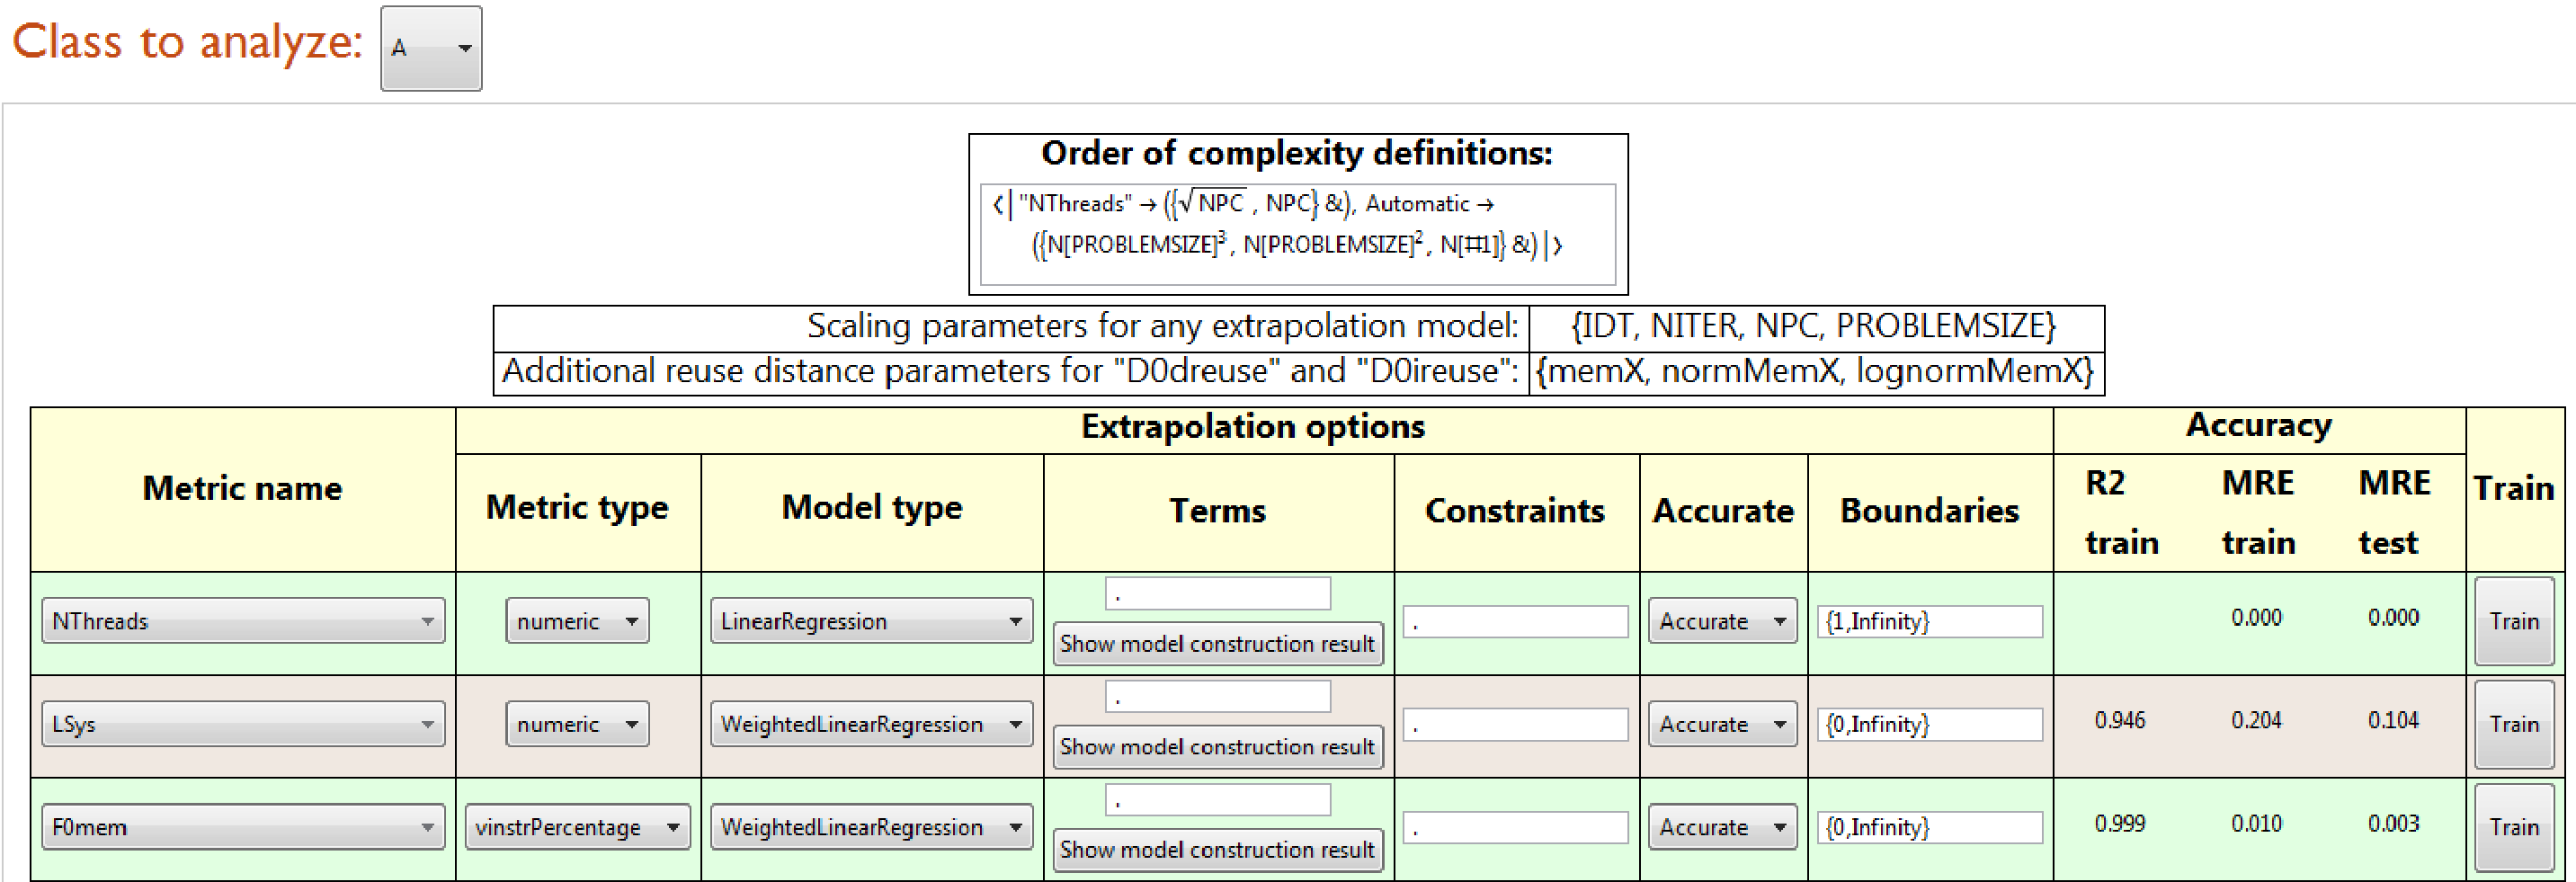
\includegraphics{./Figures/ExtrapolationListInspection.pdf}}
\caption{Upper 
side of the model inspection GUI including: the \texttt{Class to analyze} field to select the thread class
being inspected, the \texttt{Order of complexity definitions}, the list of available scaling parameters, and the heading and first few lines
of the table reporting the list of the target metrics, their model options, accuracies, and \texttt{Train} button.
}
\label{fig:extrapolationListInspection}
\end{figure}

At the bottom of the table there are the \verb!Retrain all! and \texttt{Retrain all metrics that depend on "LSys"} buttons to train
several metrics at once (either all the metrics or only the \verb!instrPercentage! and \verb!vinstrPercentage! ones).
Following these buttons we find the GUI for graphically analyzing the model behaviors (Figure \ref{fig:investigationPlots}).
To use this GUI we start from selecting the \texttt{metric to be analyzed}. There are two plots to help assessing possible misbehaviors of the model.

\begin{figure}[t!]
\centering
\resizebox{\sfigbigwhole}{!}{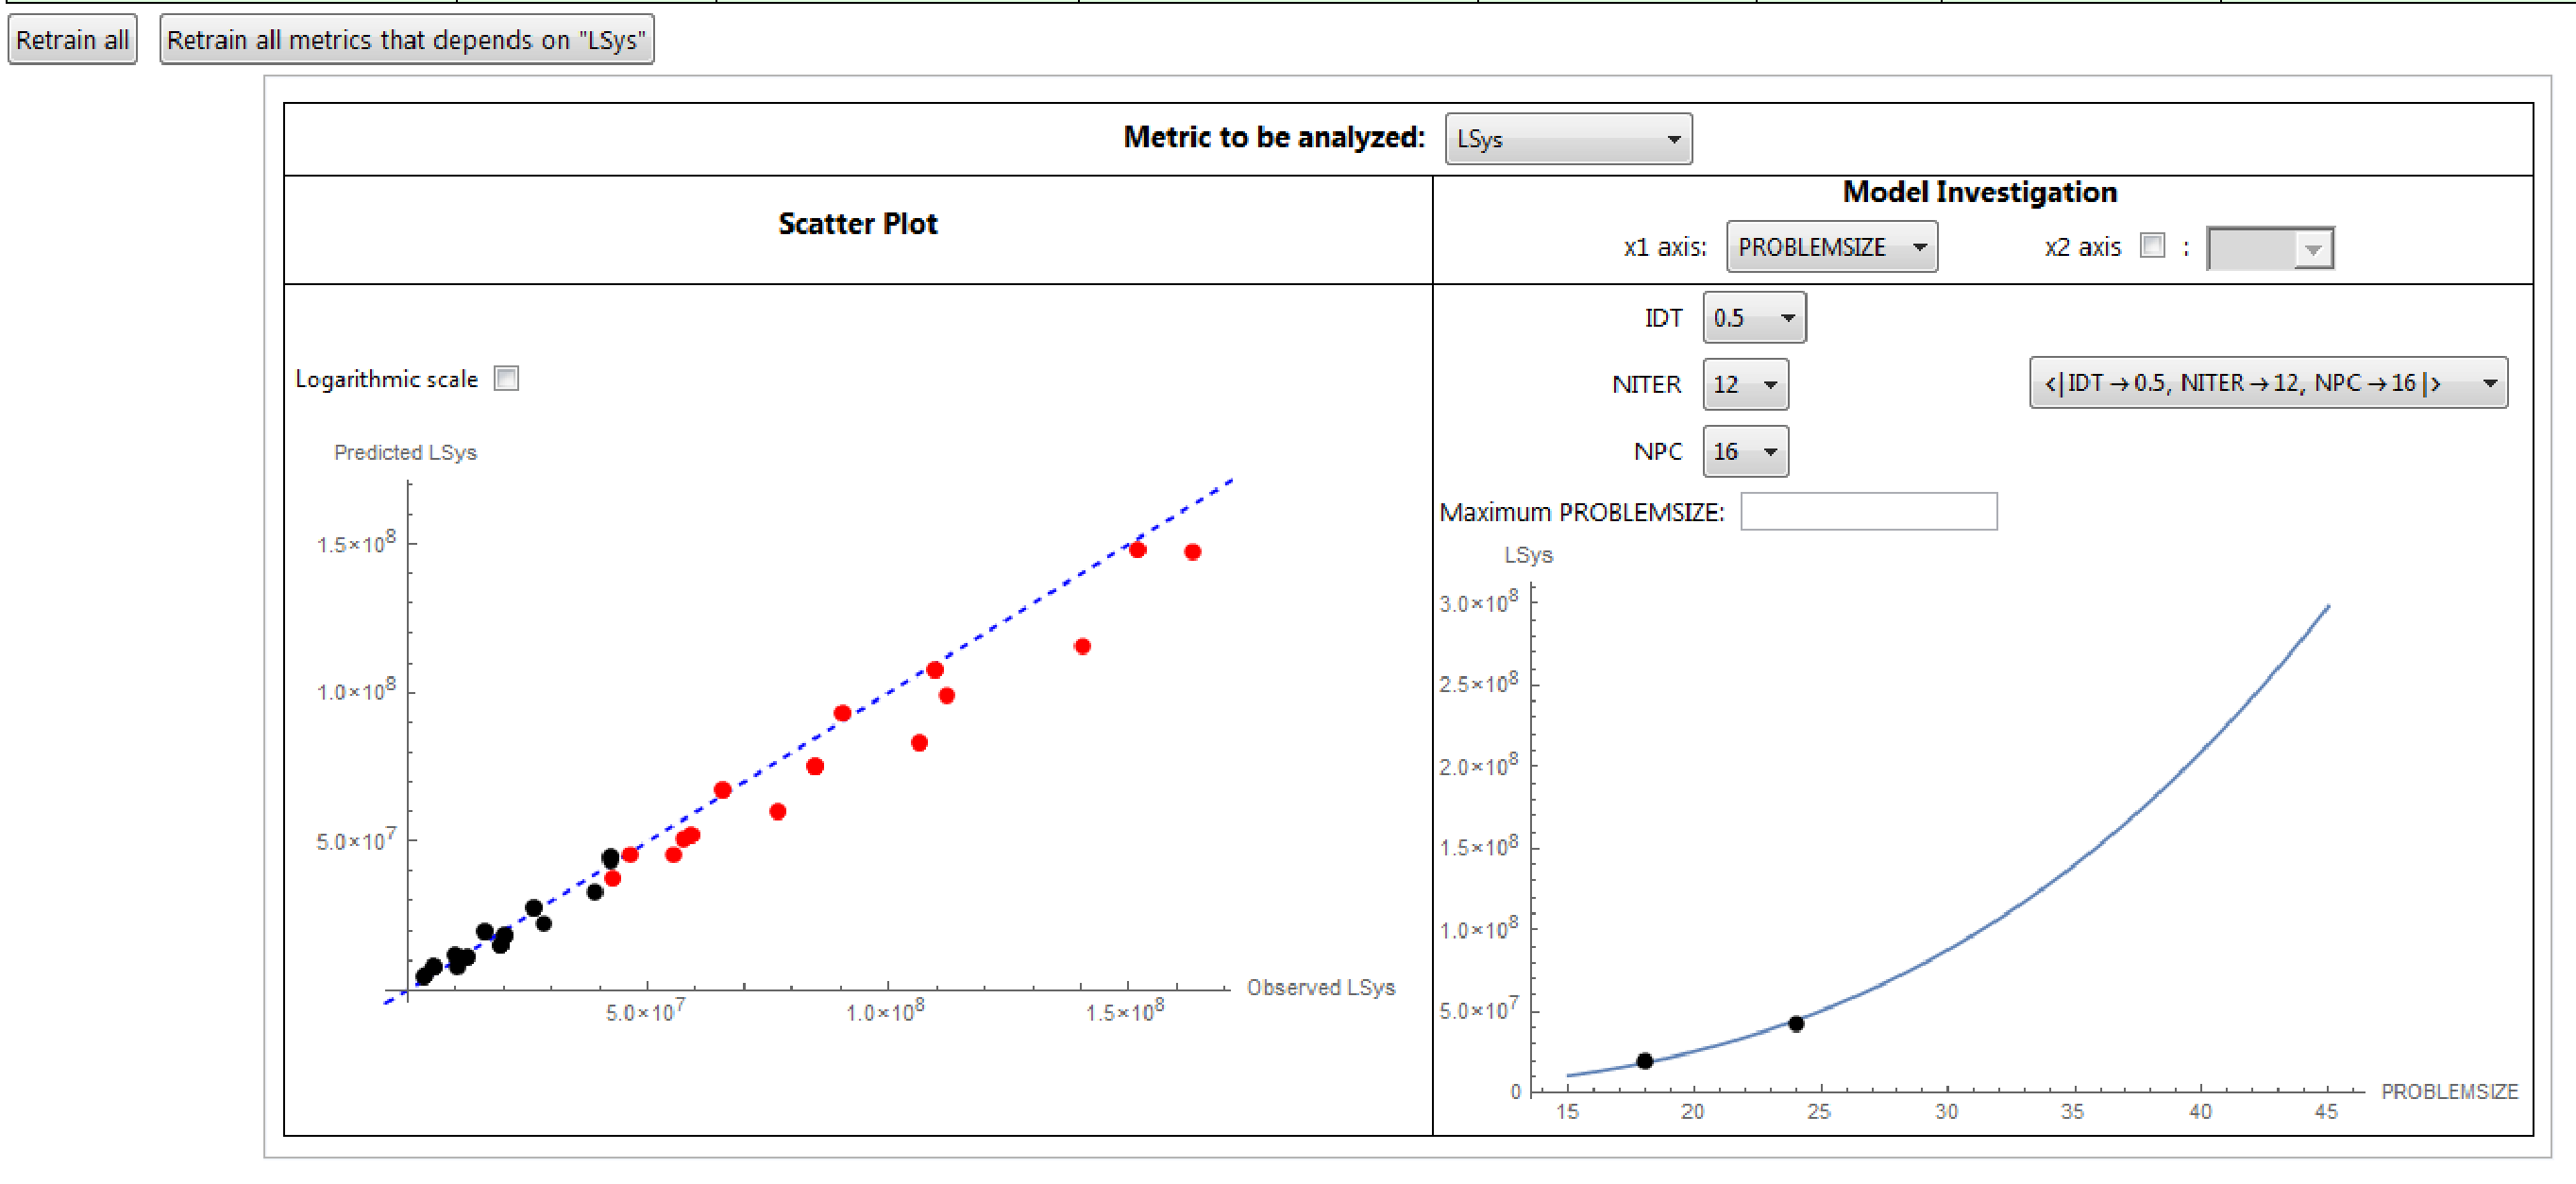
\includegraphics{./Figures/plots.pdf}}
\caption{Retrain buttons and plots to graphically access the model behavior.
}
\label{fig:investigationPlots}
\end{figure}

On the left we observe the \texttt{Scatter Plot}
that shows the trend of the observed metric with respect to the predicted one for all points in the training (black points) and test (red points)
datasets. A good model should have points lying close to the bisection shown as a dashed blue line. It is possible to show the logarithmic scale,
and for a metric \verb!m! of type \verb!vnumeric! or \verb!vinstrPercentage!,
it is also possible to switch to the visualization to the absolute count,
i.e. the product of \verb!m!$\times$\verb!LSys!, i.e. the quantity used during model construction.

On the right we can control the \texttt{Investigation Plot} to observe the trend of the predictions when varying the scaling parameters.
We can select the scaling parameter to use as independent variable and also select the values to assign to the other parameters for assessing
the model trend. In this plot, the blue line is the model prediction while the black and red dots are respectively the training and test points
(only the ones that match the selected configuration of scaling parameters are shown).
It is also possible to observe how model predictions change by varying two scaling parameters by selecting \texttt{x2 axis}.
The metric value will be shown with a color coding, the legend will be reported. In this case, if training points are observable
with the selected parameter configurations, the region where these points are available will be surrounded by black borders.

\subsection{Comments on the accuracy and visualization analysis}
The visualization in the plots and the accuracies in the table refer are computed with respect to the average metric value
along the different threads belonging to the selected class.

Note that for \textit{vectorized mix} metrics (i.e. \texttt{vnumeric} and \texttt{vinstrPercentage}),
only a single number is shown on the table for each accuracy measure. Accuracy (and metric values in the plots)
refer in this case to the aggregate number, i.e. we sum up all numbers in the metric vector representation
before the accuracy computation (and before the visualization in the plots).

\subsection{Suggestions: what metrics to inspect and how to improve a poor model?}

In theory one should check all metrics for all thread classes.
We actually recommend to briefly screen all metrics by taking a look to the accuracy numbers in the table.
All metrics whose MRE on the test (or train) set is considered unacceptable for the specific study should be inspected and possibly corrected
(few suggestions for corrections are given later in this section). We recommend also to inspect (and possibly correct)
any metric having an R2 value below 0.7.
Finally we recommend to inspect and correct (if needed) all metrics having a significant discrepancy between train and test MRE. We suggest this
because, even if the test MRE value could be considered acceptable, the discrepancy might be due to divergence between the prediction model
and the actual metric that might increase indefinitely when moving towards the extrapolation scale.

When inspecting a model we first recommend to take a look to the terms selected by the model construction by clicking on the button
\texttt{Show model construction result} in the column \texttt{Terms} of the table. This will show the list of the selected terms that we can paste
into the \texttt{Terms} field of the table by clicking the \texttt{Paste} button. Once pasted there, we can easily edit it if needed.

We analyze the trend on the plot while thinking if the suggested terms are reasonable. Note that many different models are tested
and it is not possible to exclude a priori possible overfitting and the introduction of terms that improve the quality on the training data
but not on the test data (Section \ref{sec:semiauto}). If this is the case, we would probably note some suspicious terms starting from some point of
the list. Note that the model construction starts adding the terms from the most relevant ones, thus the ones appearing last in the list 
may actually be spurious. We suggest to remove the suspicious last terms and retrain the model.

By default, all scalar metrics that are expected to be upper and lower bounded are treated as \texttt{instrPercentage}.
This has been proven to return high quality models for several applications but it is not always the case. For \texttt{ILP}
related metrics the transformation $ILP\times LSys$ has no direct physical meaning and the approach of using \texttt{instrPercentage}
is probably not sound (but empirically it seems to work pretty well). If an \texttt{instrPercentage} metric is problematic,
we recommend to try to change it to \texttt{numeric} and apply a \texttt{NeuralNetwork} model.

If a significant divergence between the actual and predicted metric is found in the plots and the above approaches are not applicable,
then we may try to reconsider the \texttt{Order of complexity definitions}. Are those definitions
actually correct? Particular care should be given to
exponential terms. In fact it is not possible to change their base by fitting a coefficient during linear regression and if the wrong base
has been entered in the complexity definitions, then the model will for sure diverge. That is: $c_1*b_1^{x} \neq (c_1*b_1)^{x} \neq c_2*b_2^{x}$, being $c_1$
and $c_2$ constant of whatever values (different from 1), and $b_1$ and $b_2$ two constant bases ($b_1\neq b_2$). Note that the same problem
does not happen with logarithms because:
\begin{eqnarray}
 c_1\log_{b_1}(x) = c_1 * \frac{\log_{b_2}(x)}{\log_{b_2}(b_1)}~~\Rightarrow~~ c_1\log_{b_1}(x) = c_2\log_{b_2}(x), \\
 c_2 = \frac{c_1}{\log_{b_2}(b_1)}.
\end{eqnarray}
Thus any base for a logarithm can be automatically compensated by a change in the constant from $c_1$ to $c_2$ from within the linear regression.

Besides possible problems with a wrong base in an exponential term, we may have forgotten (or not expected)
some polynomial terms of different orders.

Some points in the training set could have been profiled at a scale too small to observe the scaling behavior and being characterized by
some initialization process. This may lead to difficulties in the model construction that may return a poor model.
Sometimes this problem can be figured out by checking the \texttt{Scatter Plot}, some points would simply be very far from the bisection (possibly
in the logarithmic scale). In this case we should remove the problematic points and retrain all models. An expert user can remove
the points by directly editing the \texttt{ExtrAxTrainAlgInfo} from within the \ex notebook. Nevertheless we recommend to remove the profile files
from the \ex project directory and restart from pass 1.

\section{Generating the extrapolated profiles}
\label{sec:output}

The last \ex pass is the extrapolation of the algorithm profile at the target scale. This pass is implemented in Section
\textbf{Pass 6: Profile extrapolation} of the \ex notebook.
The GUI will provide an input field for each scaling parameter. Put in this input field the list of values that we want
to investigate for each parameter. The extrapolations will then be generated for all combinations
of the listed parameter values by clicking the button \texttt{Extrapolate}.
We can save the extrapolated data by using the backup button.

The data stored in the file \texttt{pass6.m} in the \ex project directory can then be used to feed the \eb analytic model.


\section{Contributors}
\label{sec:contributors}
\begin{itemize}
 \item Giovanni Mariani
 \item Rik Jongerius
 \item Gero Dittmann
 \item Andreea Anghel
\end{itemize}

\section{Acknowledgement}
\label{sec:ack}
This work is conducted in the context of the joint
ASTRON and IBM DOME project and is funded by the Dutch Ministry of Economische Zaken and the Province of Drenthe.

\appendix

\newpage

  \begin{table}[t!]
\centering
\scriptsize
%\tiny
\caption{List of fields in the JSON object describing an individual thread profile. Some of these fields could be missing in the input file. In this case,
the JSON read functionalities of \ex and \eb will show a warning and will set the internal data structure to its default value.}
% \setlength\tabcolsep{0.15cm}
  \begin{tabular}{|p{3cm} ||p{8.2cm}| }
   \hline
  \textbf{Field name} & \textbf{Description} \\
   \hline
   \hline
   \texttt{threadId} & Identifier of the OpenMP thread id. Always 0 if the application does not use OpenMP. This is a mandatory field. \\
   \hline
   \texttt{processId} & Identifier of the MPI process id. Always 0 if the application does not use MPI. This is a mandatory field. \\
   \hline
   \texttt{instructionMix} & A JSON object describing the instruction mix (Section \ref{sec:pisaImix}). \\
   \hline
   \texttt{openMPinstructionMix} & A JSON object listing the OpenMP library calls. In this object, field
   names are the OpenMP function names and the stored values are the call counters.  \\
   \hline
   \texttt{mpiInstructionMix} & A JSON object listing the calls to the MPI library (Section \ref{sec:pisaMPI}). \\
   \hline
   \texttt{ilp} & An array of JSON objects describing the application ILP (Section \ref{sec:pisaILP}). \\
   \hline
   \texttt{dataReuseDistribution} & A JSON object describing the data-memory reference-reuse distribution (Section \ref{sec:pisaReuse}). \\
   \hline
   \texttt{instReuseDistribution} & A JSON object describing the instruction-memory reference-reuse distribution (Section \ref{sec:pisaReuse}). \\
   \hline
   \texttt{memoryFootprint} & A JSON object describing the memory footprint (Section \ref{sec:pisaFootprint}). \\
   \hline
   \texttt{registerAccesses} & A JSON object storing the number of accesses to registers. \\%\texttt{reads} and \texttt{writes}
% 	whose values refer to the number of accessed registers. \\
   \hline
   \texttt{mpiDataExchanged} & Object listing the number of messages and bytes sent and received using peer to peer communication routines.
   It also includes information about collective communication requests. \\
   \hline
   \texttt{mpiCommunicationVector} & An array describing the communication received
	by the given thread (Section \ref{sec:pisaCommVector}). \\
   \hline
   \texttt{externalLibraryCallCount} & A JSON object listing the number of times every external
	function was invoked during program execution (field names are the function
	names and field values are the call counters). Note that, to support \textit{Fortran} compatibility,
	function names are case insensitive. \\
  \hline
\end{tabular}
\label{tab:pisaThreadFields}
  \end{table}


\section{Iput profile format}
\label{apx:pisaFormat}

\pisa generates output files to describe application profile in JSON.
In this Section we briefly describe the file format focusing on the data that is read by \ex and \eb.
The profile files may include additional information. The JSON field names are human readable and an example of JSON
file, \texttt{example.pisa}, is included in the \texttt{Documentation} folder of \ex and \eb.

The mandatory fields in the main JSON object are:
\begin{itemize}
 \item \texttt{application}: a string identifying the application name,
 \item \texttt{appScale}: a JSON object that lists all the application scaling parameters and their values,
 \item \texttt{threads}: an array of JSON object, each storing an individual thread profile.
\end{itemize}

The JSON object storing an individual thread profile includes the fields Listed in Table \ref{tab:pisaThreadFields}
and described in the following subsections.



\subsection{Instruction mix analysis format}
\label{sec:pisaImix}
The field \texttt{instructionMix} stores a JSON object with the following format.

It includes a field \verb!instructions_analyzed! that stores the count of the total executed instructions
(it excludes instructions executed in external libraries).

Then, for each instruction type it stores the a field named as the instruction type and that includes information about total count and detailed data on
the type of vectorization in use and type of the processed data, e.g.:

\begin{Verbatim}[obeytabs, tabsize=2, frame=lines]
				"load_instructions": [
					{
						"total_instructions": 101,
						"mix": [
							{
								"vector_size": 1,
								"float_16bits": 0,
								"float_32bits": 0,
								"float_64bits": 0,
								"float_80bits": 0,
								"float_128bits": 0,
								"float_128bits_powerpc": 0,
								"float_64bits_mmx": 0,
								"int_4bits": 0,
								"int_8bits": 0,
								"int_16bits": 0,
								"int_32bits": 101,
								"int_64bits": 0,
								"int_misc": 0,
								"struct_type": 0,
								"array_type": 0,
								"pointer_type": 0,
								"instructions": 101
							}
						],
						"scalar_instructions": 101,
						"vector_instructions": 0,
						"misc_instructions": 0
					}
				]
\end{Verbatim}

\subsection{MPI-calls analysis format}
\label{sec:pisaMPI}

For each MPI function, the counter of the number of times it has been invoked is stored.
The call counters are organized by type, additionally the overall counter is also included (\verb!MPI_instructions_analyzed!).
For example, the field \verb!collectiveCommunicationRoutines! stores the counters for all collective communication routine,
while \verb!p2pCommunicationRoutines! stores counters related to peer-to-peer communication routines.

\subsection{ILP analysis format}
\label{sec:pisaILP}
The field \verb!ilp! stores an array of objects to describe the application ILP. Each object in the array
stores ILP information collected for a different window size. Usually, only one object is stored for the window size value
of 54. For each object in the array, there are three fields: \verb!windowSize!, \verb!statistics!, and \verb!in-order!.
The \verb!statistics! and \verb!in-order! are two objects with the same structure that store information about
the estimated out-of-order ILP (\verb!statistics!) and in-order ILP (\verb!in-order!).
In each of these objects, information about the ILP and execution \texttt{span}
(the execution length in cycles assuming all single-cycle-latency instructions).
For example:
\begin{Verbatim}[obeytabs, tabsize=2, frame=lines]
					"statistics": {
						"span": 604,
						"arithmetic_mean": 2.1225,
						"span_mem": 176,
						"arithmetic_mean_mem": 1.142,
						"span_int": 601,
						"arithmetic_mean_int": 1.5723,
						"span_ctrl": 127,
						"arithmetic_mean_ctrl": 1.0708,
						"span_fp": 0,
						"arithmetic_mean_fp": 0.0
					}
\end{Verbatim}

The overall ILP is stored in the field \verb!arithmetic_mean!. Other fields named \verb!arithmetic_mean_<type>! store
the information about ILP measured independently for different instruction types.


\subsection{Reuse distance analysis format}
\label{sec:pisaReuse}

The fields \verb!dataReuseDistribution! and \verb!instReuseDistribution! store information about memory reference reuse
respectively for data and instruction memory. This data is stored in an array of objects.
We consider a memory reference to be one cache line long, thus any address accessed in the same cache-line is considered
as a single reference \cite{anghel2016}. Each object stored in the array has a
different value for the field \verb!cacheLineSize! (measured in bytes).
Objects in the array \verb!instReuseDistribution! store also a field \verb!instructionSize!
that refers to the instruction length in bytes considered during the analysis.

The field \verb!statistics! stores reuse information with two-fields objects. The field names are \verb!data! and \verb!dataCDF!
for \texttt{dataReuseDistribution}, and \verb!instructions! and \verb!instructionsCDF! for \texttt{instReuseDistribution}.
The first field stores an array where each element is a couple \verb![ <reuseDistance>, <eventCount> ]! where \verb!eventCount!
is the number of times a memory reference has been reused at a distance between the given \verb!reuseDistance! and the one appearing
in the previous couple. The latter field store an array where each element is a couple \verb![ <reuseDistance>, <cdf> ]!.

For example:
\begin{Verbatim}[obeytabs, tabsize=2, frame=lines]
			"dataReuseDistribution": [
				{
					"cacheLineSize": 128,
					"statistics": {
						"data": [
							[
								0,
								194
							],
							[
								1,
								1
							],
							[
								2,
								1
							],
							[
								4,
								1
							]
						],
						"dataCDF": [
							[
								0,
								0.9651
							],
							[
								1,
								0.9701
							],
							[
								2,
								0.9751
							],
							[
								4,
								0.98
							]
						]
					}
				}
			]
\end{Verbatim}


\subsection{Memory footprint analysis format}
\label{sec:pisaFootprint}
The field \verb!memoryFootprint! is an object storing the following fields:
\begin{itemize}
 \item \verb!shared_addresses_byte_granularity!: total bytes accessed by all OpenMP threads (including the current one),
 \item \verb!total_distinct_addresses_byte_granularity!: total number of bytes accessed by the current OpenMP thread,
 \item \verb!shared_accesses!: total cache lines accessed by all OpenMP threads (including the current one),
 \item \verb!total_distinct_accesses_starting_addresses!: total cache lines accessed by the current thread,
 \item \verb!cache_line_size!: the considered cache line size in bytes. 
\end{itemize}



\subsection{Communication vector format}
\label{sec:pisaCommVector}
The field \verb!mpiCommunicationVector! is an array of objects each to store data about the MPI communication received by the
current process from other MPI processes. Each object stores three fields:
\begin{itemize}
 \item \verb!source! the MPI process id of the source process,
 \item \verb!received_bytes! total size of data received from the given source,
 \item \verb!received_messages! total messages received from the given source.
\end{itemize}

Only peer-to-peer communications are taken into account.
An example:
\begin{Verbatim}[obeytabs, tabsize=2, frame=lines]
	"mpiCommunicationVector": [
		{
		  "source": 0,
		  "received_bytes": 148480,
		  "received_messages": 224
		},
		{
		  "source": 2,
		  "received_bytes": 148736,
		  "received_messages": 226
		},
		{
		  "source": 5,
		  "received_bytes": 156880,
		  "received_messages": 225
		}
	]
\end{Verbatim}

\section{\ex data structure}

\subsection{Mathematica format of application profiles}
\label{apx:matheAppFormat}

Application profiles read from input files are stored in the variables \verb!ExtrAxTrainAlgInfo! and \verb!ExtrAxTestAlgInfo!
within the \ex notebook (within the \eb notebook the variable \verb!ExaBoundsAlgInfo! is used). Once the extrapolation
are generated in pass 6 (Section \ref{sec:output}), the variable \verb!predictedAlgorithm! will have the same format
to store the predicted profiles.

These variables are \mathe associations that map application names to their \textit{execution information}.
\textit{Execution information} are \mathe associations with a key \verb!scalingParameters! (associated to the list of scaling parameters)
and one additional key for each \textit{scaling configuration} mapped to the profiles observed for that scaling configuration.
A \textit{scaling configuration} is a \mathe association that maps each scaling parameter with its value. Scaling parameters in
a scaling configuration are sorted alphabetically.

The functions \verb!GetScalingParameters!, \verb!GetScalingConfigurations!, and \verb!GetScalingConfigurationsHaving! can be used
to access \textit{execution information}.


Some examples:
\begin{itemize}
 \item \verb!GetScalingParameters[ ExtrAxTrainAlgInfo["LU"] ]!: returns the list of scaling parameters for the application \verb!"LU"!,
 \item \verb!GetScalingConfigurations[ ExtrAxTestAlgInfo["LU"] ]!: returns the list of all scaling configurations
 in the test set (\verb!ExtrAxTestAlgInfo!) of the application \verb!"LU"!,
 \item \verb!GetScalingConfigurationsHaving[ predictedAlgorithm["LU"], <|"NPC"->100|> ]!:
 returns the list of scaling configurations
 in the extrapolated results (\verb!predictedAlgorithm!) of the application \verb!"LU"! where \verb!"NPC"! is 100.
\end{itemize}

To retrieve the profile data structure for the first scaling configuration of an application whose name is stored in
\texttt{appName} the following code can be used:
\begin{Verbatim}[obeytabs, tabsize=4, frame=lines, numbers=left]
 sc = GetScalingConfigurations[ExtrAxTrainAlgInfo[appName]][[1]];
 profiles = ExtrAxTrainAlgInfo[appName][sc];
 profile = profiles[[1]];
\end{Verbatim}

Line 1 assigns to the variable \verb!sc! the first scaling configuration in the training set of the application \verb!appName!.
Line 2 assigns to \texttt{profiles} the list of all profiles collected for the given scaling configuration \verb!sc!.
Note that the data structure supports the possibility of storing information of multiple executions for the same scaling configuration.
This allows an analysis of the variability in the different metrics. Thus at Line 2, \texttt{profiles} store
a list of all the profiled runs (\ex makes use only of the first run and does not
account for the others). Line 3 assigns to \verb!profile! the profile data associated to the first run.
These three lines can be used to access \verb!ExtrAxTestAlgInfo! or \verb!predictedAlgorithm! by replacing \verb!ExtrAxTrainAlgInfo!
with one of those variables.

The \verb!profile! data is an association whose keys are thread identifiers and values are the profiled metrics for that thread.
The thread identifier is a couple \verb!{<processId>, <threadId>}! if the profile is taken from
\verb!ExtrAxTrainAlgInfo! or \verb!ExtrAxTestAlgInfo!. For \verb!predictedAlgorithm! the association keys
are actually class identifier in string format (e.g. \verb!"cluster<classId>"!, class ids are natural
numbers starting from 1).
In this case, a metric named \verb!NThreads! will be stored along the different profiled metrics to indicate the number of threads belonging to
this class.

The profile stored for a thread (or a thread class) is a list of key-value pairs: \verb!{<metricName>, <metricValue>}!.
The list of metric names and their meaning are listed in Appendix \ref{apx:metricList}, and the structure of the metric values
are described in Appendix \ref{apx:matheMetricFormat}.

It is possible to access to a value of a given metric by using the function: 

\verb!GetKeyValue[profile,metricName]!

where \verb!metricName! should be a variable storing the metric name.
For convenience, it is possible to convert a list of key-value pairs into an association and vice-versa by using the functions:
\verb!KeyValueList2Association!, and \verb!Association2KeyValueList!.


\subsection{Mathematica format of metric types}
\label{apx:matheMetricFormat}
As mentioned in Section \ref{sec:mType}, there are three basic metric types that can be extrapolated by \ex:
\textit{scalar}, \textit{vectorized mix}, and \textit{memFunction}.
In a key-value pair \verb!{<metricName>, <metricValue>}!, the basic type of the metric defines the structure of \textit{metricValue}.
Additionally there is a forth metric type that can be used for classification but whose extrapolation model has not been implemented,
this is the \textit{communication vector} type.

For \textit{scalar} metrics, \verb!metricValue! is a number.

For \textit{vectorized mix} metrics, \verb!metricValue! is a list of lists.
Each sublist has two elements, the first one is a number that represent a vector length.
The second element is a list which elements are two-elements lists whose first value is the data length and second value is the metric value
for the given vector and data lengths.
The vector lengths \verb!{1, 2, 4, 8, 16}! are listed. The data lengths \verb!{0, 4, 8, 16, 32, 64, 128}! are listed and refer to the lengths
in bits of the data type.
The length of 0 bits refers to data types whose lengths are unknown at instrumentation-time.
In fact, \pisa instruments directly the LLVM-IR before processing it through the compiler back-end. Some data types have machine-specific lengths
that will be known only when executing the compiler back-end.

The following example shows the structure of a \textit{vectorized mix} metric:
\begin{Verbatim}[obeytabs, tabsize=4, frame=lines]
{
	{1, {
				{0, 0.0000271334}, {4, 0.}, {8, 4.34135*10^-6}, {16, 0.},
				{32, 0.00500151},{64, 0.175334}, {128, 0.}
			}
		},
	{2, {
				{0, 0.}, {4, 0.}, {8, 0.}, {16, 0.},
				{32, 0.}, {64, 0.0178644}, {128, 0.}
			}
		},
	{4, {
				{0, 0.}, {4, 0.}, {8, 0.}, {16, 0.},
				{32, 0.}, {64, 0.}, {128, 0.}
			}
		},
	{8, {
				{0, 0.}, {4, 0.}, {8, 0.}, {16, 0.},
				{32, 0.}, {64, 0.}, {128, 0.}
			}
		},
	{16, {
				{0, 0.}, {4, 0.}, {8, 0.}, {16, 0.},
				{32, 0.}, {64, 0.}, {128, 0.}
			}
		}
}
\end{Verbatim}

For \textit{memFunction} metrics, \verb!metricValue! is a list of two-elements lists being the first element a reuse distance and the second one
its CDF value. All reuse distances at power of two levels are always stored (up to the maximum observed reuse distance). Other reuse distance values
are optionals. An example is the following:
\begin{Verbatim}[obeytabs, tabsize=4, frame=lines]
{
	{1, 0.2255}, {2, 0.3693}, {4, 0.5895}, {5, 0.6463}, {8, 0.7486},
	{9, 0.8132}, {10, 0.8335}, {13, 0.8661}, {15, 0.872}, {16, 0.8744},
	{17, 0.8782}, {18, 0.8829}, {21, 0.8886}, {22, 0.8904}, {23, 0.8915}, 
	{28, 0.9005}, {29, 0.901}, {30, 0.9015}, {31, 0.902}, {32, 0.9025}
}
\end{Verbatim}

The only \textit{communication vector} metric is named \texttt{MPIcommVector}. This metric is a list of triples \texttt{<relativeSrc>,<size>,<msgs>},
where \texttt{<relativeSrc>} is the number to be added to the MPI process id of the current thread to compute the id the process
source of the communication, \texttt{<size>} is the amount of data received from that source, and \texttt{<msgs>} is the number of messages
received. For example the structure \verb!{{1, 57400, 145}, {5, 57368, 145}}! represents the fact that the current process \verb!<processId>!
receives messages from two processes, the first one with id \verb!<processId>+1! and the second one with \verb!<processId>+5!. The value of 
\texttt{<relativeSrc>} is always positive. If \verb!<processId>+<relativeSrc>! exceeds the total number of processes \verb!<totProcess>! in the application run,
the id of the process source of the communication can be computed as \texttt{(<processId>+<relativeSrc>)\%<totProcess>}, where \% is the modulus operator.
\texttt{MPIcommVector} accounts only for peer-to-peer communications.



\subsection{Mathematica format of classification data}
\label{apx:clusteringStructure}

During the \textbf{Pass 2: Thread classification} in the \ex notebook we classify the thread profiles (Section \ref{sec:classification}).

Classification data is stored in the variables \texttt{classificationTrain} and \texttt{classificationTest}. The testing data does
not take active role when learning the classification function but, once the classification function is learnt upon the training data,
this classification is applied to the test data to generate \texttt{classificationTest}.

The variables \texttt{classificationTrain} and \texttt{classificationTest} are \mathe associations whose keys are
the application names. The value associated to the target application is in turn an association with the following fields:
\begin{itemize}
 \item \verb!"clusterStructure"!: An association with keys the scaling configurations and values the clustering results.
 Clustering results are a nested list with, as first level the application run
 (multiple runs with the same scaling configurations are supported in this data structure). The second level is the cluster.
 The third level is the two-elements thread identifier.
 For example: \verb!{{{{0, 0}}, {{1, 0}, {2, 0}, {3, 0}}, {{4, 0}}}}! describes a clustering result for a scaling configuration executed only once
 (the first level of the list has a single element). In the example there are 3 clusters (the second level has 3 elements). The first
 cluster includes only the thread having MPI process id 0. The second cluster includes the MPI processes 1, 2, and 3. The third cluster includes
 MPI process 4. All OpenMP thread ids are 0.
 
 This data is always accessible regardless the classification method in use. The clusters are sorted consistently
 along the different scaling configurations
 accordingly to their classification.
 
 \item \verb!"reducedStructure"!: An association with keys the scaling configurations and with values the profile structure
 in the reduced dimension space obtained using principal component analysis. The profile structure is a list whose elements are
 profiles for different application runs (carried out at the given scaling configuration). for a given run, the profile is organized in an
 association where keys are thread identifiers and values are lists of metric-value pairs. The metric names in this case are \verb!"PCA<n>"!
 with \texttt{n} from 1 up to the number of PCA components selected by applying the Kaiser's criterion.
 
 This structure is not set up when using the \texttt{communication pattern regularity analysis} method. In that case there will appear a single
 PCA (\verb!"PCA1"!) with a constant 0 value.
 
 \item \verb!"absoluteEdgeMatching"!: A data structure storing the results of the vote propagation mechanism
 used to propagate the classification along different scaling configurations \cite{mariani201Xclassification}.
 It is an association whose keys are pairs of scaling configurations. The first scaling configuration in the pair is the voting configuration,
 while the second is the voted one. The values are the voted sorting of the clusters. For example:
 \texttt{\{<|"NPC" -> 25, 
   "PROBLEMSIZE" -> 15|>, <|"NPC" -> 16, 
   "PROBLEMSIZE" -> 18|>\} -> \{1, 2, 3, 4\}} implies that the vote from the first scaling configuration to the second one agrees with the current
   classification, i.e. the first class has been voted as first etc.. A vote such as
 \texttt{\{<|"NPC" -> 25, 
   "PROBLEMSIZE" -> 15|>, <|"NPC" -> 16, 
   "PROBLEMSIZE" -> 18|>\} -> \{1, 2, 4, 3\}} implies that the current classification differs with the given vote
   and the third class has been voted as being the forth one. A discordant vote can happen because the final classification is obtained by using a
   majority voting scheme and minority votes can exist.
 
 This structure is not set up when using the \texttt{communication pattern regularity analysis} method. In that case, \verb!"absoluteEdgeMatching"!
 is an empty association.
 
 \item \verb!"threadDimensionReducer"!: A function that takes as argument a thread profile and returns as a result its description in the
 reduced PCA space.
 
 When the \texttt{communication pattern regularity analysis} method is used, the stored function always returns  0.
 
 \item \verb!"commGroupsClusterStructure"!: An association with keys the scaling configurations and with values a list of communication groups \cite{wu2012}
 data structure.
 Each communication group is an association with the following fields:
 \begin{itemize}
 \item \verb!"startRank"!: the id of the first MPI process belonging to the group.
 \item \verb!"dimensions"!: the geometric dimensions of this group.
 \item \verb!"dimension<n>"!: one of this field for each dimension. It is an association including two fields: \verb!iterations!, and \verb!stride!.
 MPI process ids of processes belonging to this communication group are organized in sequence with the given stride repeated for the given
 number of iterations. If multiple dimensions are involved, then they are sorted in ascending order of stride. To compute all the ids, starting from
 the startRank, apply the stride and iterations of the first dimension to obtain a set of ids. Then apply to each of this ids the stride of the second dimension
 for the required number of iterations. And so on.
 \item \verb!"communicationVector"!: a list of associations. Each association describes the communication coming from another process and includes: 
 \verb!"relativeSrc"! number to be added to the process id to compute the id of the process source of the communication,
 \verb!"minSize"! minimum amount of data size received by any process member of this communication group from the source computed with the given relative id,
 \verb!"maxSize"!, \verb!"medianSize"!, \verb!"meanSize"!, \verb!"stdevSize"!,
 \verb!"minMsgs"! minimum number of messages received by any process member of this communication
 group from the source computed with the given relative id, \verb!"maxMsgs"!, \verb!"medianMsgs"!,
 \verb!"meanMsgs"!, \verb!"stdevMsgs"!.
 \end{itemize}
 
 
 This field is not present when using the \texttt{general communication and processing analysis} method.
 
 \textbf{For predicting the communication pattern and thus the metric \texttt{MPIcommVector}, one must start from here.
The trend of: \texttt{startRank}, \texttt{iterations} and \texttt{stride} (for each dimensions), and the content of each element of
each communication vector has to be predicted as a function of the scaling parameters.
Note that, in the package \texttt{CommunicationPatternClustering}, the function \texttt{ExplodeCommGroup} can be used to pass from a communication group
data structure to the complete list of MPI process ids belonging to the group.
 }
 \item \verb!"commGroupsClusterStructure"!: returns the options to be passed to the function \texttt{MultiplerunsThreadClusteringGUI}
 to reproduce the current classification.
\end{itemize}



\subsection{Mathematica format of extrapolation models}
\label{apx:extrapolationModel}

In the \ex notebook, the extrapolation model is stored in the variable: \texttt{extrapolationModel}.
Once generated through \textbf{Pass4}, this variable is structured as an association whose keys are
the class identifiers and whose values are lists of extrapolation models for the target metrics.

An extrapolation model of a target metric is an association with the following keys:
\begin{itemize}
 \item \verb!"metricName"!, the metric name.
 \item \verb!"metricType"!, the metric type as described in Section \ref{sec:mType}.
 \item \verb!"heteroscedasticityCompensation"!, the function selected for compensating heteroscedasticity.
 \item \verb!"predictorNames"!, list of the names of the predictor variables necessary for querying the model.
 \item \verb!"predictorTerms"!, the terms used by the model (Section \ref{sec:terms}). These are the model selection results
 (or the ones specified by the user if the model selection has not been carried out).
 \item \verb!"modelType"!, the model type (Section \ref{sec:modelType})
 \item \verb!"model"!, the function implementing the model.
 Where each element is a target scaling configuration represented by the value the \verb!predictorTerms!.
 It returns as output a list of predicted metrics, one for each target scaling configuration.
 \item \verb!"posNmonotonConstraints"!, the user-defined monotonicity constraints (Section \ref{sec:Constraints}).
 \item \verb!"maxMemModel"!, the model generated to predict the maximum reuse distance.
 \item \verb!"knotMemModels"!, a list of other prediction models that could be used to predict the reuse distance that
 would return a certain CDF value. This is not used in general.
 \item \verb!"boundaries"!, the metric boundaries (Section \ref{sec:boundaries}).
\end{itemize}


  \begin{table}[t!]
\centering
\scriptsize
%\tiny
\caption{List of predefined \ex metrics, their expected type, their short description and whether they are required by \ex and \eb or optional.}
% \setlength\tabcolsep{0.15cm}
\begin{tabular}{|p{3.8cm} | p{1.5cm} ||p{7.6cm}| p{1.7cm} |}
\hline
\textbf{Name} &\textbf{Type} & \textbf{Decscription} & \textbf{Required} \\
\hline
\hline
\texttt{NThreads} &\texttt{scalar} & Number of threads in a class & Required \\
\hline
\texttt{LSys} &\texttt{scalar} & Total instruction count & Required \\
\hline
\texttt{F0mem} &\texttt{vectorized mix} & fraction of memory instructions (load plus store) & Required \\
\hline
\texttt{F0load} &\texttt{vectorized mix} & fraction of load instructions & Required \\
\hline
\texttt{F0store} &\texttt{vectorized mix} & fraction of store instructions & Required \\
\hline
\texttt{F0addr} &\texttt{vectorized mix} & fraction of memory address-computation instructions & Required \\
\hline
\texttt{F0int} &\texttt{vectorized mix} & fraction of all instructions using the integer ALU (includes bitwise logical instructions and conversion instructions) & Required \\
\hline
\texttt{F0intOnly} &\texttt{vectorized mix} & fraction of arithmetic integer instructions & Optional \\
\hline
\texttt{F0intmul} &\texttt{vectorized mix} & fraction of integer multiplications & Required \\
\hline
\texttt{F0intdiv} &\texttt{vectorized mix} & fraction of integer divisions & Required \\
\hline
\texttt{F0fp} &\texttt{vectorized mix} & fraction of floating point instructions & Required \\
\hline
\texttt{F0fpmul} &\texttt{vectorized mix} & fraction of floating point multiplications & Required \\
\hline
\texttt{F0fpdiv} &\texttt{vectorized mix} & fraction of floating point divisions & Required \\
\hline
\texttt{F0control} &\texttt{vectorized mix} & fraction of control flow instructions & Required \\
\hline
\texttt{F0vector} &\texttt{vectorized mix} & fraction of vector-management operations (insert, extract, shuffle) & Required \\
\hline
\texttt{F0other} &\texttt{vectorized mix} & other miscellaneous operations & Required \\
\hline
\texttt{D0dreuse} &\texttt{memFunction} & data reuse distance cumulative distribution function
(considering cache line size of 64 bytes unless otherwise specified) & Required \\
\hline
\texttt{D0dreuse128} &\texttt{memFunction} & data reuse distance cumulative distribution function
(considering cache line size of 128 bytes) & Optional \\
\hline
\texttt{D0ireuse} &\texttt{memFunction} & instruction reuse distance cumulative distribution function & Required \\
\hline
\texttt{F0bestMispredict} &\texttt{memFunction} & best-case branch misprediction probability & Required \\
\hline
\texttt{H0branch} &\texttt{scalar} & run-time entropy of the control flow & Required \\
\hline
\texttt{ILP0} &\texttt{scalar} & instruction level parallelism & Required \\
\hline
\texttt{ILP0mem} &\texttt{scalar} & instruction level parallelism for memory instructions & Required \\
\hline
\texttt{ILP0int} &\texttt{scalar} & instruction level parallelism for integer instructions & Required \\
\hline
\texttt{ILP0control} &\texttt{scalar} & instruction level parallelism for control flow instructions & Required \\
\hline
\texttt{ILP0fp} &\texttt{scalar} & instruction level parallelism for floating point instructions & Required \\
\hline
\texttt{F0regreads} &\texttt{scalar} & average number of registers read by an instruction & Required \\
\hline
\texttt{F0regwrites} &\texttt{scalar} & average number of registers written by an instruction & Required \\
\hline
\texttt{MPIinstructions} &\texttt{scalar} & total calls to the MPI library & Optional \\
\hline
\texttt{MPIisend} &\texttt{scalar} & total calls to the MPIisend & Optional \\
\hline
\texttt{MPIirecv} &\texttt{scalar} & total calls to the MPIirecv  & Optional \\
\hline
\texttt{MPIsend} &\texttt{scalar} & total calls to the MPIsend  & Optional \\
\hline
\texttt{MPIrecv} &\texttt{scalar} & total calls to the MPIrecv  & Optional \\
\hline
\texttt{MPIbcast} &\texttt{scalar} & total calls to the MPIbcast  & Optional \\
\hline
\texttt{MPIbarrier} &\texttt{scalar} & total calls to the MPIbarrier  & Optional \\
\hline
\texttt{MPIreduce} &\texttt{scalar} & total calls to the MPIreduce  & Optional \\
\hline
\texttt{MPIsentBytes} &\texttt{scalar} & total data sent through peer-to-peer MPI functions & Required \\
\hline
\texttt{MPIrecvBytes} &\texttt{scalar} & total data received with peer-to-peer MPI functions & Required \\
\hline
\texttt{MPIsentMessages} &\texttt{scalar} & total messages sent through peer-to-peer MPI functions & Required \\
\hline
\texttt{MPIrecvMessages} &\texttt{scalar} & total messages received with peer-to-peer MPI functions & Required \\
\hline
\texttt{MPIcommVector} &\texttt{communication vector} & total messages received with peer-to-peer MPI functions & extrapolation not supported \\
\hline
\texttt{OpenMPtotal} &\texttt{scalar} & total calls to the OpenMP library & Optional \\
\hline
\texttt{OpenMPsynchronization} &\texttt{scalar} & total calls to OpenMP synchronization routines & Optional \\
\hline
\texttt{OpenMPatomic} &\texttt{scalar} & total calls to OpenMP atomic routines & Optional \\
\hline
\texttt{OpenMPstartupShutdown} &\texttt{scalar} & total calls to OpenMP startup and shutdown routines & Optional \\
\hline
\texttt{OpenMPparallel} &\texttt{scalar} & total calls to OpenMP parallelization routines & Optional \\
\hline
\texttt{OpenMPthreadInfo} &\texttt{scalar} & total calls to OpenMP thread information routines & Optional \\
\hline
\texttt{OpenMPworkSharing} &\texttt{scalar} & total calls to OpenMP work-sharing routines & Optional \\
\hline
\texttt{OpenMPthreadPrivateDataSupport} &\texttt{scalar} & total calls to OpenMP thread private data support routines & Optional \\
\hline
\texttt{OpenMPtaskingSupport} &\texttt{scalar} & total calls to OpenMP tasking support routines & Optional \\
\hline
\texttt{OpenMPothers} &\texttt{scalar} & total calls to OpenMP miscellaneous routines & Optional \\
\hline
\end{tabular}
\label{tab:metrics}
  \end{table}

\section{\ex known metrics}
\label{apx:metricList}
Table \ref{tab:metrics} lists the metrics predefined in \ex.
To add a metric to the ones managed by the classification methodology and also to make sure it is correctly processed through \ex,
add the new metric declaration in the variables \texttt{metricTypeOptions} in the package:

\verb!AlgorithmExtrapolation/SingleThreadExtrapolation.m!

Besides that, one must make sure to correctly include the new metric into the application profile data structure (Appendix \ref{apx:matheAppFormat}).

\bibliographystyle{ieeetr}
\bibliography{ExtrAx}
% \bibliography{../../../../Documentation/biblio}

\end{document}
